\chapter{Background} \label{cha:Background}
This section contains the technical background for this thesis where we first introduce \ac{mmWave} specific cellular communications technology aspects in \Cref{Millimeter wave communication}. In \Cref{Channel Modeling}, the focus is on channel modeling, highlighting the differences between \ac{LOS} and \ac{NLOS} conditions. \Cref{Metasurfaces} provides a comprehensive introduction to the technology concept of metasurfaces that are envisioned to be active components of future sixth-generation (6G) radio access networks, but passive variants may already be employed in conjunction with fifth-generation (5G) networks. We then introduce existing \ac{IRS} channel models that are taken into consideration for further reinterpretation. Lastly, based on previously presented related works, \Cref{Related Work or Scope of Thesis} formulates the aims of this master thesis.
\section{Millimeter Wave Communication} \label{Millimeter wave communication}
Globally, the demand for 5G networks is rising quickly. The wireless communication of upcoming generations needs to be improved to meet our constantly increasing demand for faster data speeds and lower latency. Applications such as the \ac{IoT}, augmented reality, and driverless vehicles necessitate higher performance networks to function successfully and deliver a smooth user experience \cite{BANAFAA2023245, Towards6G}. To keep up with these growing requirements and ensure that wireless networks can meet future demands, new technology is required. The much-needed scalable increases in network capacity and peak data rates can be achieved using \ac{mmWave} communication technology. Due to more hostile propagation characteristics in terms of higher atmospheric absorption and increased susceptibility to obstacles and environmental conditions, the move to directional communications necessitates for compensating the additional path loss. Due to this, cellular mmWave communications will be drastically different from those of the current typically sub-6 GHz networks. These variations make it harder to use \ac{mmWave} communications to their fullest potential, as discussed in this section.

In typical commercial mobile wireless telecommunication systems, wireless and mobile systems operate in a specific frequency band within the sub-\SI{6}{\giga\hertz} spectrum. However, these frequency bands are saturated as a result of the exponential growth in network data traffic in current wireless communication. According to recent studies by \cite{diakhate2019propagation}, the bandwidth currently present in the sub-\SI{6}{\giga\hertz} spectrum, which is covered by 5G \ac{FR1}, will not be sufficient to achieve the capacity required for the upcoming systems.
\begin{figure}[H]
	\centering
	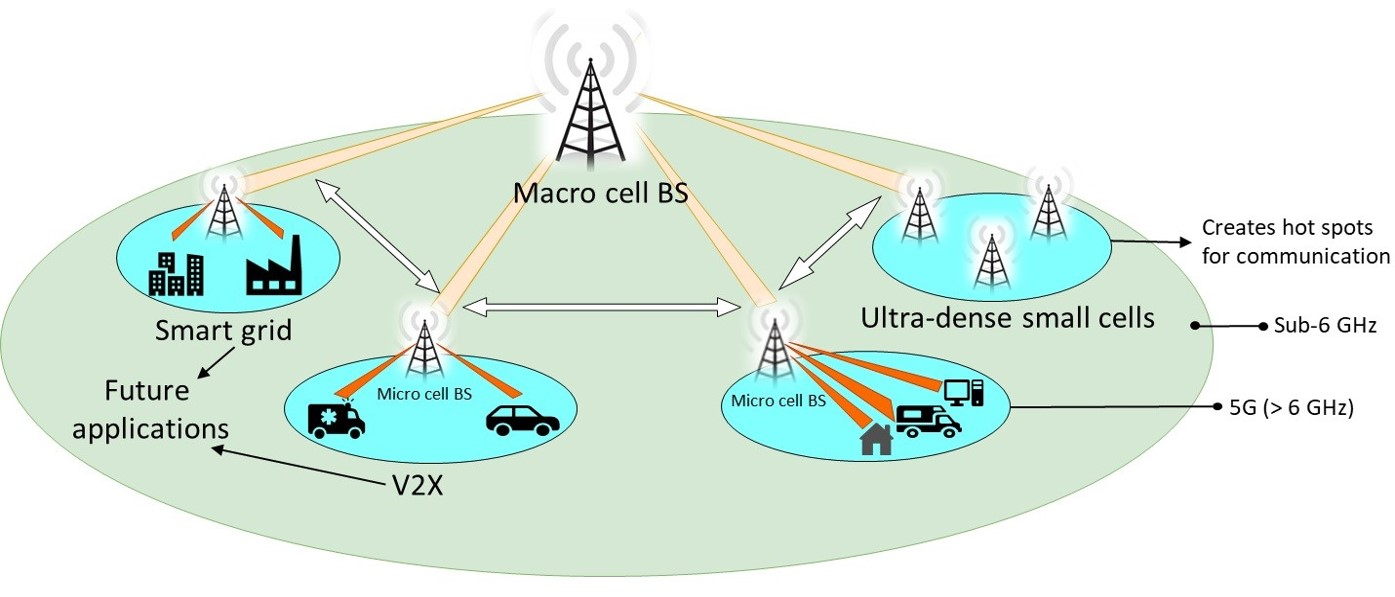
\includegraphics[width=1.0\linewidth]{images/Section 2 Images/5Gmm}
	\caption{Illustration of typical deployment of mmWave communications with use cases and future applications with the communication established between macrocell base stations at sub-\SI{6}{\giga\hertz} to the microcell base stations \cite{mmWavefig1, Sakaguchi2017WhereWA}.}
	\label{fig:5gmm}
\end{figure}
The \ac{mmWave} frequency band, which offers greater frequency bandwidths, enters the picture at this point. The \ac{3GPP} supports an additional frequency range with 5G, so-called \ac{FR2} that includes seven operational bands between \SI{24.2}{\giga\hertz} and \SI{71}{\giga\hertz}, namely n\num{257}, n\num{258}, n\num{259}, n\num{260}, n\num{261}, n\num{262}, and, n\num{263} \cite{3GPP17}. However, not all frequencies are included because, depending on the nation, only the ranges between \num{24.25}-\SI{29.5}{\giga\hertz}, \num{37}-\SI{43.5}{\giga\hertz}, \num{47.2}-\SI{48.2}{\giga\hertz}, and \num{57}-\SI{71}{\giga\hertz} shall be used.More frequency ranges have recently been identified for 6G \cite{3GPP17}, including \ac{FR4} which covers the frequency range of \SI{71}{\giga\hertz} to \SI{114.2}{\giga\hertz} and is anticipated to be used for autonomous and connected vehicles under the umbrella of \ac{ITS}. The \ac{FR5} category includes frequencies above \SI{114.2}{\giga\hertz}. Additionally, \ac{FR3} covers the majority of the space between \ac{FR1} and \ac{FR2}, i.e., the "No Man's Land" \cite{Qualcomm} between \SI{10}{\giga\hertz} to \SI{20}{\giga\hertz}. As a result, with FRs \num{2}–\num{5}, it is possible to see how crucial the spectrum above \SI{6}{\giga\hertz} will be for future communication networks.

\Cref{fig:5gmm} depicts a typical mmWave communication deployment with several use cases. We see communication linkages formed in both the sub-\SI{6}{\giga\hertz} and greater than \SI{6}{\giga\hertz} frequency ranges in this illustration. The deployment also includes ultra-dense tiny cells specifically placed to generate communication hotspots. In terms of future applications, the figure suggests smart grid and V2X (Vehicle-to-Everything) connectivity. These developing application cases demonstrate mmWave technology's adaptability and disruptive promise in enabling not only better mobile broadband but also critical infrastructure and intelligent transportation systems.

The \ac{mmWave} spectrum is expected to be used by future mobile radio networks to deliver higher data rates for novel use cases like \ac{XR}. Virtual reality, autonomous vehicles, swift factory robots, and 8K video streaming are some additional cutting-edge services made possible by \ac{mmWave} technology.
\subsection{Propagation Characteristics of mmWave} \label{Characteristics of 5G mmWave}
The \ac{EM} waves with a wavelength $\lambda$ of \SI{1}{\milli\meter} to \SI{10}{\milli\meter} are known as \ac{mmWave}. Using the formula $\ f = \frac{c}{\lambda}$, where $c$ is the speed of light $ (\approx \num{3} \cdot \SI{e8}{\meter}/\si{\second})$, we convert the wavelength to obtain a frequency range of \SI{30}{\giga\hertz} to \SI{300}{\giga\hertz}. \ac{mmWave} is also referred to as the \ac{EHF} band or the \ac{UHF} band, according to the \ac{ITU} \cite{ITU_EHF}. From an industry perspective, frequencies above \SI{20}{\giga\hertz}, sometimes even from above \SI{10}{\giga\hertz}, are also referred to as \ac{mmWave}.

So far, we have emphasized the advantages of \ac{mmWave} technology, namely that it allows for high network capacity that is future-proof and peak user data rates because of the wide available bandwidth. However, there are also drawbacks to using \ac{mmWave} frequencies. Before the adoption of 5G, frequency bands above \SI{6}{\giga\hertz} were thought to be unsuitable for mobile wireless communications due to their susceptibility to high path losses, especially as a result of obstruction by any objects, including buildings, people, and vegetation \cite{6GWireless}. At various frequencies and distances, the path loss calculations show how frequency affects wireless communication. The path loss is roughly \SI{92.4}{\decibel} at a frequency of \SI{2}{\giga\hertz} and a distance of \SI{100}{\meter}. In contrast, the path loss dramatically rises to almost \SI{108.5}{\decibel} at a higher frequency of \SI{28}{\giga\hertz}. This represents a large difference of roughly \SI{16.1}{\decibel}. When comparing a concrete wall to a similar wall at lower frequencies, the penetration loss at \SI{28}{\giga\hertz} through the wall may be much larger, up to about \SI{30}{\decibel}. Furthermore, compared to absorption losses at lower frequencies, the human body is predicted to experience a greater path loss at \SI{28}{\giga\hertz}, possibly approaching \SI{20}{\decibel}.

Environmental factors include increased atmospheric absorption, a greater impact by rain and snow, increased penetration losses, and, increased diffuse scattering due to surface roughness becoming relatively large compared to the wavelength \cite{6GWireless}. While these obstacles restrict the use of \ac{mmWave}, improved antenna technology has been suggested to make up for the extra losses with the idea of grouping numerous, now smaller, antennas into arrays that are then used for beamforming.
\subsection{Beamforming and Beam Management} \label{Beam Steering and Management}
As \ac{mmWave} has short wavelengths and high frequencies, antennas get smaller and can be combined into antenna arrays with a small form factor. Through the use of beamforming and such antenna arrays, the antenna directivity is made possible in a specific direction. This will be used for transmission and reception. There, the impact of significant path loss can be lessened or even mitigated by the beamforming gain. The formed beam can be configured in any way, but the idea is to direct the resulting antenna beam along the strongest propagation path for maximum efficiency. In addition, the antenna pattern can have some directions nulled to lessen interference from/at other devices. A multi-armed antenna beam may also be realized to serve multiple users, depending on the hardware architecture. When two or more antenna elements are arranged spatially and electrically in arrays that are connected, directional radiation patterns can be created. The feed network, which refers to the connections between the RF front end and the antenna elements, creates a phased array by assigning each element a phase. To improve the received signals, adjustments may even be made to the amplitude of the individual antenna branches \cite{Ali2017BeamformingTF}. The individual antenna elements' radiation patterns, mounting orientations, and polarizations as well as the geometry of the array all have an impact on how well the array works.

Because wireless communication frequently serves mobile users, the beam directions must be continuously aligned. Beam management processes include beam tracking and beam switching techniques for sustaining the established link. With slight adjustments, the former constantly modifies the Tx and Rx beam orientation. This dynamic alignment is critical for overcoming the hurdles given by mobile users' changing position, and maintaining a stable and high-quality connection. Beam tracking allows the system to monitor the user's location and modify the beam direction in real time to maintain the best possible link. Beam-switching techniques, in addition to beam tracking, play an important part in seamless communication by permitting smooth transitions between available propagation paths and base stations when the user's movement necessitates such handovers \cite{s23094359, 8947954}. These beam management approaches are critical for delivering the performance and dependability that current wireless communication systems demand.
\section{Channel Modeling } \label{Channel Modeling}
Channel modeling is an essential part of the design of efficient wireless communication systems. To design a communication system that performs reliably and effectively, we need a process to characterize and optimize its behavior based on its fundamental mathematical representation of the physical channel \cite{Rappaport, rappaport2015millimeter}. Thus, the representation of how transmitted EM waves interact with the environment is one of the core values of channel modeling. The properties such as free-space path loss and interactions with objects in terms of reflection, diffraction, and scattering are modeled \cite{rappaport2015millimeter, electronics12092014}. Moreover, the antenna patterns of the transmitter and receiver are considered. These are quantifiable, making it possible to predict the channel conditions in particular environments. As we delve further into this subject, we investigate various channel modeling methodologies, approaches, and tools that are used to fully comprehend the \ac{mmWave} communication environment and its effect on system performance.

A Tx and Rx scenario is succinctly illustrated in \Cref{fig:TxRx}, which also shows the LOS path to the receiver at Rx1 with gain $G_{Rx1}$ and NLOS path to the receiver at Rx2 with gain $G_{Rx2}$ from the transmitter Tx with gain $G_{Tx}$. To enhance this illustration, a sample Channel Impulse Response (CIR) is shown on the right, providing a practical understanding of how the channel response could seem for both LOS and NLOS paths with some amount of propagation delay. The time-varying reaction of a communication channel to an impulse signal is represented by the channel impulse reaction, which effectively characterizes the features of the channel \cite{ITUReport}.

\begin{figure}[tb]
	\centering
	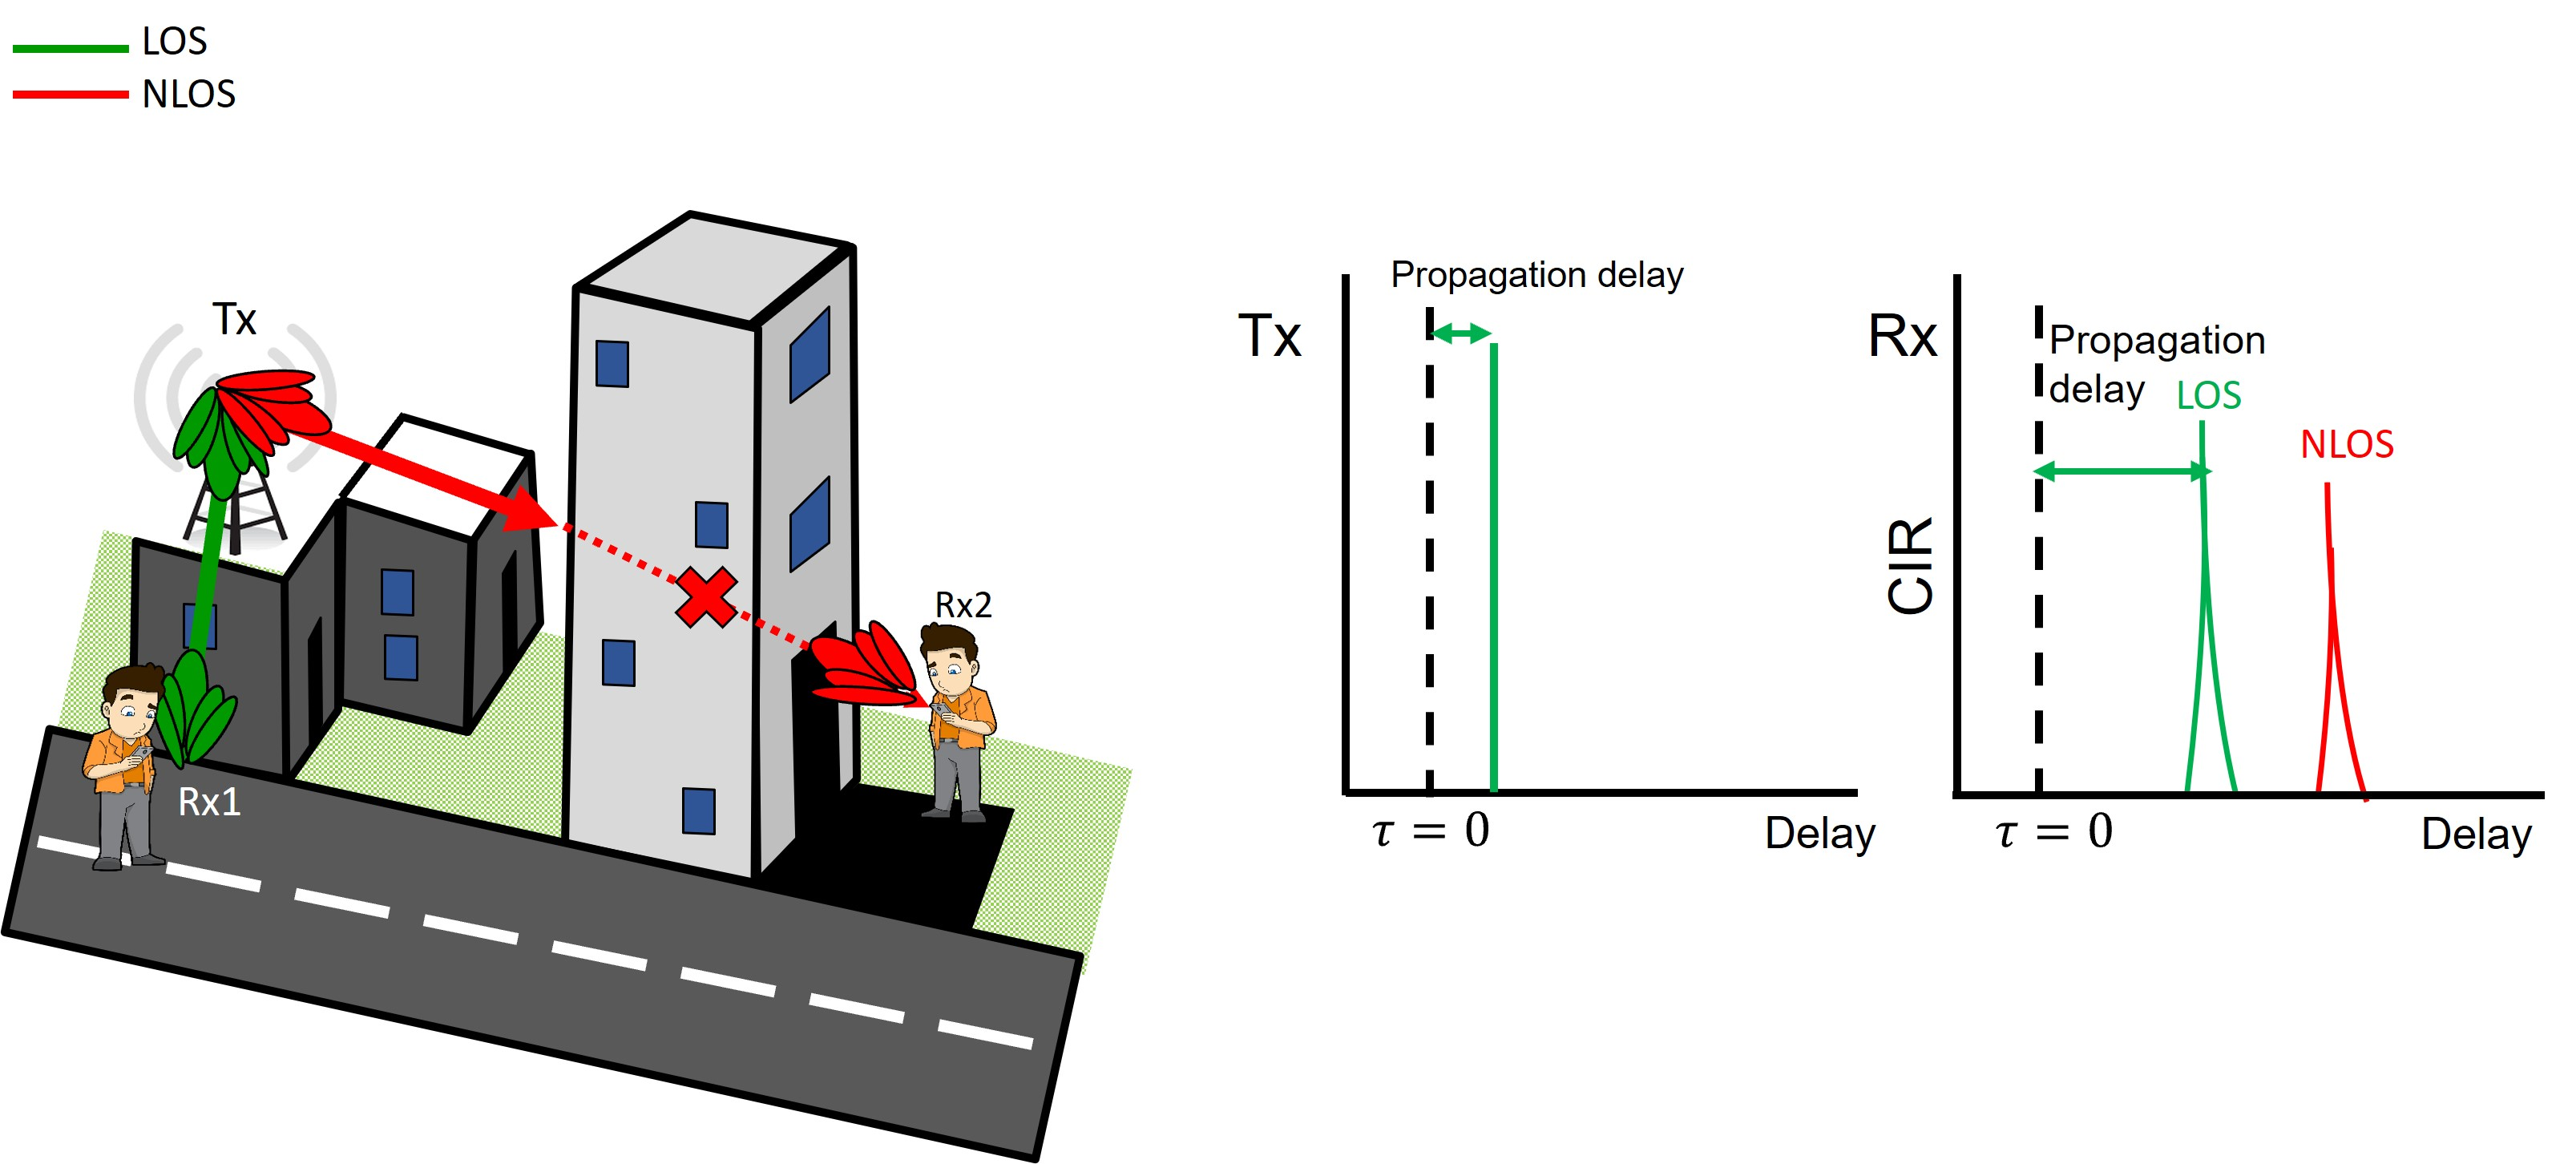
\includegraphics[width=1.0\linewidth]{images/Section 2 Images/TxRx}
	\caption{Illustration of a simple communication system with the transmitter Tx with gain $G_{Tx}$ in LOS path with Rx1 with gain $G_{Rx1}$ and NLOS path with Rx2 with gain $G_{Rx2}$. The sample CIR graphs on the right include both the LOS and NLOS paths for the general grasp of the idea \cite{ITUReport}.}
	\label{fig:TxRx}
\end{figure}
\subsection{Propagation Environment} \label{Propagation Environment}
Many different channel modeling techniques can be used in this setup for system and network planning \cite{KabulUni, 3GPP17}. Popular models include WINNER and COST, and as the world transitions to \ac{mmWave}s, models from the \ac{3GPP}, \ac{ITU}, and IEEE are becoming increasingly important. A brief overview of existing schemes is followed by a detailed introduction of a few channel models \cite{diakhate2019propagation}.

The suitability or applicability of channel models depends on those traits. Others are restricted to 2D propagation, while some cannot be used at \ac{mmWave}s because they only take into account sub-\SI{6}{\giga\hertz} frequencies. The computationally difficult and labor-intensive modeling alternative to any such method is ray-tracing which simulates the propagation of EM waves in a particular environment \cite{rappaport2015millimeter,sun2018propagation} by following rays from the transmitter to the receiver and accounting for reflections, diffraction, and scattering \cite{pen}. Stochastic modeling is a form of statistical modeling, that uses probability distributions to describe the channel properties based on measurements or ray-tracing simulations. With these types of models, whether \ac{LOS} or \ac{NLOS} conditions are present is frequently a crucial parameter for path loss prediction.

\Cref{Mmwave Channel modeling efforts by different organizations} provides an overview of such available mmWave channel models. A hybrid propagation model that combines the previously described deterministic and stochastic elements serves as the foundation for the few-channel model. The deterministic component uses ray-tracing to simulate the spread of radio waves by following each individual ray as it interacts with various elements of the environment. To take into account the randomness and variability in the propagation environment, the stochastic component is based on statistical models \cite{8207426}. Apart from these, 3GPP propagation models are empirical, i.e., they extract characteristics that describe radio wave propagation in various situations from real-world measurement data.
\begin{table}[tb] % H -> dieses objekt wird genau da wo der code steht festgenagelt
	\footnotesize
	\caption{\ac{mmWave} channel modeling efforts by different organizations with their operating frequencies and the kind of propagation models that they support.}
	\label{Mmwave Channel modeling efforts by different organizations}
	\centering
	\begin{tabular}{C{3.25cm}|C{1.3cm}|C{1.8cm}|C{0.7cm}|C{2.3cm}|C{1.7cm}|C{1.9cm}}
		\textbf{Channel Model} & \bf Source & \bf Frequency & \bf Year & \bf Environment & \bf Mobility Support & \bf Propagation Models \\
		\hline 
		\ac{5GCM} & \cite{5GCM, KabulUni} & \SI{28}{\giga\hertz}, \SI{38}{\giga\hertz}, \SI{73}{\giga\hertz} & \num{2011} & Indoor, outdoor & Yes & Hybrid\\
		\hline 
		\ac{METIS} &  \cite{METIS, KabulUni} & up to \SI{100}{\giga\hertz} &  \num{2012} & Indoor, outdoor & No & Hybrid \\
		\hline 
		Third Generation Partnership Project (\ac{3GPP}) & \cite{3GPP17, KabulUni} & up to \SI{100}{\giga\hertz} &  \num{2017} & Indoor, outdoor & Yes & Empirical\\
		\hline 
		\ac{MiWEBA} & \cite{miwebaquadriga, weiler2016quasi} & \SI{60}{\giga\hertz} &  \num{2014} & Outdoor & No & Stochastic \\
		\hline 
		\ac{QuaDRiGa} & \cite{miwebaquadriga} & \SI{30}{\giga\hertz} & \num{2014} & Indoor, outdoor & Yes & Hybrid \\
	\end{tabular}
\end{table}
Because these models are the result of intensive field testing and measurement, they are useful instruments for forecasting signal behavior and enhancing mobile communication system performance. In the following sections, we consider alternative channel models. The free-space path loss model is first introduced in \Cref{Free space propagation model} and then followed up by the 3GPP UMi and UMa models in \Cref{3GPP channel model}.
\subsection{Free-Space Propagation Model} \label{Free space propagation model}
The FSPL model constitutes the fundamental and most simplistic channel model considering a radio signal in free space, i.e., there is LOS between Tx and Rx and no multipath propagation. \Cref{Eq:Free space propagation} describes the received power in free-space conditions.
\begin{equation} \label{Eq:Free space propagation}
	P_{Rx}= P_{Tx} \frac{G_{Tx} \cdot G_{Rx} \cdot \lambda^2 }{(4 \cdot \pi \cdot r_{Tx, Rx})^2}
\end{equation}
Here $P_{Tx}$ and $P_{Rx}$ are the transmitted and received power in Watts, respectively, $r_{Tx, Rx}$ is the 3D \ac{LOS} distance between the transmitter and the receiver, $G_{Tx}$ and $G_{Rx}$ are the gains of the transmitter and receiver antennas relative to an isotropic radiator with a unit gain, and $\lambda$ is the wavelength of the carrier in \si{\meter} \cite{9205413}.

Accordingly, the power loss between $P_{Tx}$ and $P_{Rx}$ is referred to as propagation path loss $PL_{dB}$, as depicted in  \Cref{Eq:path loss formula}. Combining \Cref{Eq:Free space propagation} and \Cref{Eq:path loss formula}, and moving from linear to decibel presentation, we provide the logarithmic FSPL channel model in the FSPL in  \Cref{equation1}. \Cref{fig:fspl} depicts the relation between path loss in \si{\decibel} as a function of Tx-Rx distance $r_{Tx, Rx}$ in \si{\meter}. 
\begin{equation} \label{Eq:path loss formula}
	PL_{dB}= 10\cdot \log_{10} \left( \frac{P_{Tx}}{P_{Rx}} \right) 
\end{equation}
\begin{equation} \label{equation1}
	PL_{dB}= -147.5 \; \si{\decibel} + 20 \cdot  \log_{10} \left(\frac{r_{Tx, Rx}}{\SI{1000}{\meter}} \right) + 20 \cdot \log_{10} \left(\frac{f}{\SI{1000}{\mega\hertz}}\right) + G_{Tx, dB} + G_{Rx, dB}
\end{equation}
\begin{figure}[tb]
	\centering
	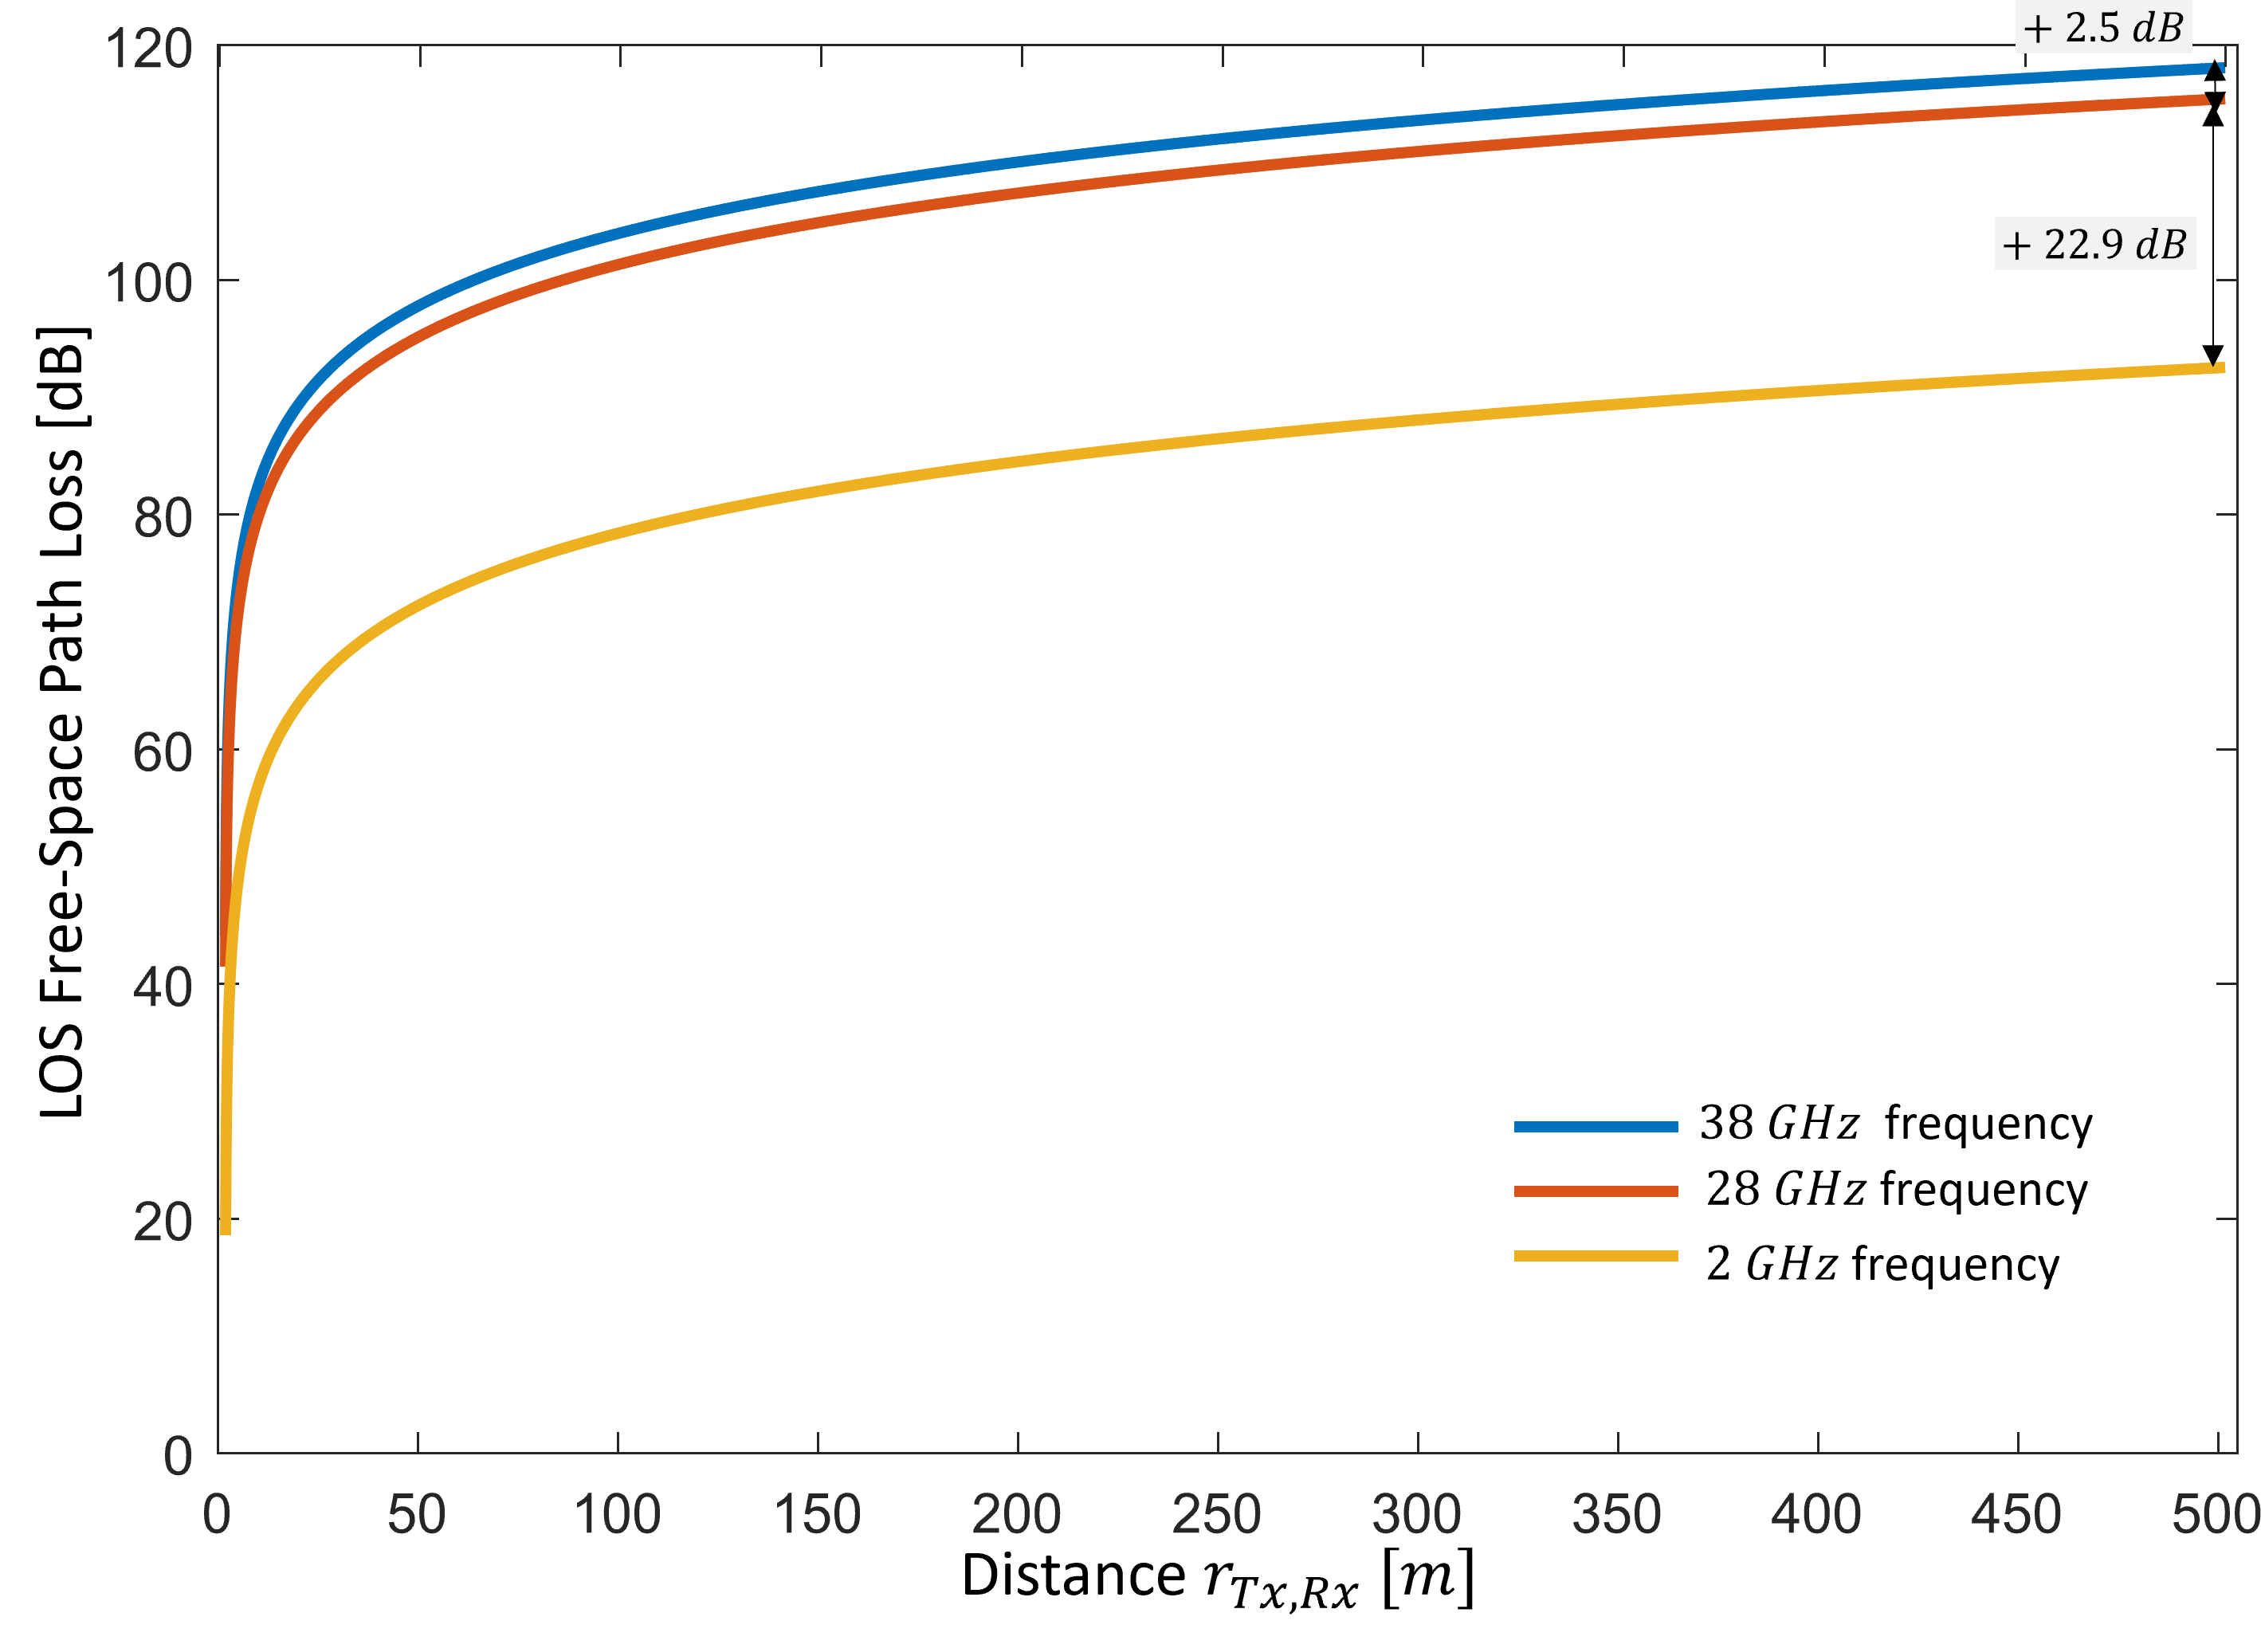
\includegraphics[width=0.8\linewidth]{images/Section 2 Images/fspl}
	\caption{Free-space path loss propagation in \si{\decibel} as a function of Tx-Rx distance in \si{\meter} for the \ac{LOS} condition at \SI{38}{\giga\hertz}, \SI{28}{\giga\hertz}, and \SI{2}{\giga\hertz} frequency. A notable decrease in the path loss is observed as the frequencies decrease.}
	\label{fig:fspl}
\end{figure}
For the increase in Tx-Rx distance, the exponential curve depicts the inverse proportionality relation between received power and the path loss. The figure also depicts the variation in path loss curves for different frequencies: \SI{38}{\giga\hertz}, \SI{28}{\giga\hertz}, and \SI{2}{\giga\hertz}, where we observe path loss differs by more than \SI{2.5}{\decibel} and \SI{22.9}{\decibel} between these three curves. Hence, the antenna gains $G_{Tx}$, and $G_{Rx}$ must be sufficiently large to compensate for these higher losses.
\begin{equation} \label{FSPL_Linear_Radar}
	P_{Rx_{Radar}}= P_{Tx} \cdot \frac{G_{Tx} \cdot G_{Rx} \cdot \lambda^2 \cdot \sigma_{Meta}}{(4 \cdot \pi)^3 \cdot (r_{Tx, Ref})^2 \cdot (r_{Ref,Rx})^2}
\end{equation}
In the case of obstructions, a virtual LOS is established where the combined path loss from Tx to the reflector and from the reflector to Rx is no longer necessary as a different path passes via Tx-reflector-Rx. To address this, we present the notion of radar path loss in \Cref{FSPL_dB_Radar} in logarithmic scale, which is developed from radar power received in \Cref{FSPL_Linear_Radar}.
\begin{equation} \label{FSPL_dB_Radar}
	\begin{aligned}
%		PL_{FSPL_{Radar}}(r_{Tx,Ref},r_{Ref,Rx},f,\sigma_{Meta},G_{Tx}, G_{Rx})&=PL_{FSPL}(G_{Tx}, r_{Tx,Ref},f)+PL_{FSPL}(G_{Rx}, r_{Ref,Rx},f)+\\ &\sigma_{Meta}-\Delta D_{ChainnedFSPL}\\
		PL_{FSPL_{Radar}}&= -136.5 \; \si{\decibel}+ 20\cdot log_{10}(r_{Tx, Ref})+ 20\cdot log_{10}(r_{Ref, Rx})+ 20 \cdot log_{10}(f)\\
		& - \sigma_{Meta}  + G_{Tx, dB} + G_{Rx, dB}
	\end{aligned}
\end{equation}
Here, $\sigma_{Meta}$ is the gain at the reflecting metasurface. This method effectively conveys the essence of instances using virtual LOS. The FSPL model implicitly assumes that there are no obstructions that the EM wave can interact with, this is very different from terrestrial communications, where there are obstructions like ground and building reflections as well as obstructions like building, human, or vegetation penetration losses, radar equations can be used. Although the FSPL model is a helpful starting point for understanding signal propagation, it should be noted that it is a simplified representation and thus might not accurately depict real-world scenarios. 
\subsection{3GPP Channel Model} \label{3GPP channel model}
For greater accuracy in terrestrial situations, we employ more sophisticated propagation models or EM simulations such as ray-tracing. In the next section, we introduce key \ac{3GPP} channel models and their boundary conditions, giving an illustration of a straightforward model applicable to 5G communication scenarios on Earth. To address the diversity of 5G deployment scenarios in wireless communication systems, the \ac{3GPP} has defined several channel models. The \ac{UMi} and \ac{UMa} are two widely used models that capture the characteristics of urban and suburban areas, respectively.
\subsubsection{UMi Channel Characterization} \label{UMi channel characterization}
The radio propagation characteristics in UMi environments are represented by the \ac{3GPP} UMi model, as summarized in \Cref{UMi scenario}. It applies to urban areas with a high user density, small cell sizes, and a mix of indoor and outdoor users. To account for the important effects that carrier frequency and antenna heights have on the signal propagation characteristics in urban microcell deployment scenarios, find a channel model description suitable for such scenarios operating at various frequency bands, such as sub-\SI{6}{\giga\hertz} and \ac{mmWave}. Path loss equations for the \ac{LOS} and \ac{NLOS} are given by \Cref{UMi_LOS} and \Cref{UMi_NLOS}, respectively. This channel model uses shadow fading $\sigma_{SF}$ of \SI{4}{\decibel} for \ac{LOS}, and \SI{7.82}{\decibel} for \ac{NLOS} conditions. The applicability range for receiver $h_{Rx}$ lies between \SI{1.5}{\meter} to \SI{22.5}{\meter} and the transmitting antenna height by default is \SI{10}{\meter} with an \ac{ISD} of up to \SI{500}{\meter} \cite{ETSI}. The applicability frequency ranges for path loss formulas are from \SI{0.5}{\giga\hertz} < $f$ < \SI{100}{\giga\hertz}. \Cref{UMi scenario}  consists of a break point distance $d_{BP}$, given by $d_{BP}= 4 \cdot h_{Tx} \cdot h_{Rx} \cdot \frac{f}{c}$, where after the path loss increases additionally as partial obstruction likelihood becomes more likely.
\begin{table}[H] % H -> dieses objekt wird genau da wo der code steht festgenagelt
	\caption{UMi path loss model for LOS and NLOS conditions with their applicability parameters that can be deemed to be suitable for many scenarios as defined by 3GPP \cite{ETSI}.}
	\footnotesize
	\label{UMi scenario}
	\centering
	\begin{tabular}{c|c|c|c}
		\textbf{Modality} & \bf Path Loss [dB]  & \begin{tabular}{@{}c@{}}\textbf{Shadow Fading} \\ \textbf{Standard Deviation [\si{\decibel}]}\end{tabular} & \begin{tabular}{@{}c@{}}\textbf{Condition} \\ \textbf{Parameters} \end{tabular} \\
		\hline
		LOS & 
		\begin{tabular}{@{}c@{}c@{}}
			\begin{equation} \label{UMi_LOS}	
				PL_{UMi-LOS} = 
				\begin{cases}
					PL_1 & \SI{10}{\meter} \leq r_{Tx, Rx} \leq d_{BP}\\
					PL_2  & d_{BP} \leq r_{Tx, Rx} \leq \SI{5}{\kilo\meter}	
				\end{cases}
			\end{equation}
			\\
			\begin{equation}
				PL_1 = 32.4  + 21 \cdot \log_{10}(r_{Tx, Rx})+ 20 \cdot \log_{10}(f)
			\end{equation}
			\\
			\begin{equation}
				\begin{aligned}
					PL_2 &= 32.4 + 40 \cdot \log_{10}(r_{Tx, Rx})+ 20\cdot \log_{10}(f)\\
					&-9.5\cdot \log_{10}\left( (d_{BP})^2 + (h_{Tx}-h_{Rx})^2 \right)
				\end{aligned}
			\end{equation}
		\end{tabular}
		& $\sigma_{SF}=4$  &
		\begin{math}
			\begin{aligned}
				\SI{1.5}{\meter} & \leq h_{Rx} \leq \\ &\SI{22.5}{\meter}\\
				h_{Tx} &=\SI{10}{\meter}}
		\end{aligned}
	\end{math}\\[10ex]
	\hline
	NLOS & 
	\begin{tabular}{@{}c@{}}
		\begin{equation} \label{UMi_NLOS}
			PL_{UMi-NLOS} = \max( PL_{UMi-LOS}, PL`_{UMi-NLOS})
		\end{equation} \\
		for $\SI{10}{\meter} \leq r_{Tx, Rx} \leq \SI{5}{\kilo\meter}$
		\\
		\begin{equation}
			\begin{aligned}
				PL`_{UMi-NLOS} &= 22.4 +35.3\cdot \log_{10}(r_{Tx, Rx})\\ 
				& +21.3\cdot \log_{10}(f)- 0.3(h_{Rx}-1.5)
			\end{aligned}
		\end{equation}
	\end{tabular}
	& $\sigma_{SF}=7.82$  &
	\begin{math}
		\begin{aligned}
			\SI{1.5}{\meter} & \leq h_{Rx} \leq \\ &\SI{22.5}{\meter}\\
			h_{Tx} &=\SI{10}{\meter}
		\end{aligned}
	\end{math}
\end{tabular}
\end{table}
The UMi channel model characterizes characteristics common in close-range urban microcell scenarios for short distances $r_{Tx, Rx}< \SI{10}{\meter}$. This setting results in increased path loss, which amplifies the impacts of multipath effects and produces noticeable channel impairments. The model does a good job of portraying the difficulties involved with small-scale urban deployments. However, the UMi model might not be the best option for longer distances, like \SI{5}{\kilo\meter}. UMi is primarily designed for short-range applications in urban environments, and its accuracy decreases with increasing distance from the cell center. In these cases, as the communication range goes beyond the model's specified design parameters, one might expect an increase in path loss and a commensurate decrease in signal quality.
\subsubsection{UMa Channel Characterization} \label{UMa channel characterization}
Analog to the UMi channel model, the \ac{3GPP} defines the \ac{UMa} model for urban macrocell deployments with the characteristics presented in \Cref{UMa scenario}. Path loss equations for the \ac{LOS} and \ac{NLOS} are given by \Cref{UMa_LOS} and \Cref{UMa_NLOS}, respectively.

The differences to the previously described model are as follows: the model uses shadow fading of \SI{4}{\decibel} for \ac{LOS} and \SI{6}{\decibel} for \ac{NLOS} conditions. The applicability range for the receiver lies between \SI{1.5}{\meter} to \SI{22.5}{\meter} and transmitting antenna height by default is \SI{25}{\meter}.


UMa is designed with macro cellular scenarios in mind, with a focus on wide coverage across greater areas. There may be relatively little path loss for distances $r_{Tx, Rx}< \SI{10}{\meter}$ inside the cell service area. Nonetheless, the unique features of the urban macro environment have a significant impact on the channel conditions. However, UMa performs better over longer distances, like five kilometers and has a moderate path loss than UMi since it is designed to mimic the channel conditions found in macrocells, which cover large areas.

\begin{table}[H] % H -> dieses objekt wird genau da wo der code steht festgenagelt
	\caption{UMa path loss model for LOS and NLOS conditions with their applicability parameters that can be deemed to be suitable for many scenarios as defined by 3GPP \cite{ETSI}.}
	\footnotesize
	\label{UMa scenario}
	\centering
	\begin{tabular}{c|c|c|c}
		\textbf{Modality} & \bf Path Loss [dB]  & \begin{tabular}{@{}c@{}}\textbf{Shadow Fading} \\ \textbf{Standard Deviation [\si{\decibel}]}\end{tabular} & \begin{tabular}{@{}c@{}}\textbf{Condition} \\ \textbf{Parameters} \end{tabular} \\
		\hline
		LOS & 
		\begin{tabular}{@{}c@{}c@{}}
			\begin{equation} \label{UMa_LOS}	
				PL_{UMa-LOS} = 
				\begin{cases}
					PL_1 & \SI{10}{\meter} \leq r_{Tx, Rx} \leq d_{BP}\\
					PL_2  & d_{BP} \leq r_{Tx, Rx} \leq \SI{5}{\kilo\meter}	
				\end{cases}
			\end{equation}
			\\
			\begin{equation}
				PL_1 = 28 + 22 \cdot \log_{10}(r_{Tx, Rx})+ 20 \cdot \log_{10}(f)
			\end{equation}
			\\
			\begin{equation}
				\begin{aligned}
					PL_2 &= 28 + 40 \cdot \log_{10}(r_{Tx, Rx})+ 20 \cdot \log_{10}(f)\\
					&- 9 \cdot \log_{10} \left( (d_{BP})^2 + (h_{Tx}-h_{Rx})^2 \right)\\
				\end{aligned}
			\end{equation}
		\end{tabular}
		& $\sigma_{SF}=4$  &
		\begin{math}
			\begin{aligned}
				\SI{1.5}{\meter} & \leq h_{Rx} \leq \\ &\SI{22.5}{\meter}\\
				h_{Tx} &=\SI{25}{\meter}
			\end{aligned}
		\end{math}\\[10ex]
		\hline
		NLOS & 
		\begin{tabular}{@{}c@{}}
			\begin{equation} \label{UMa_NLOS}
				PL_{UMa-NLOS}= \max( PL_{UMa-LOS}, PL`_{UMa-NLOS})
			\end{equation} \\
			for $\SI{10}{\meter} \leq r_{Tx, Rx} \leq \SI{5}{\kilo\meter}$
			\\
			\begin{equation}
				\begin{aligned}
					PL`_{UMa-NLOS} &= 13.54 + 39.08\cdot \log_{10}(r_{Tx, Rx})\\
					&+ 20 \cdot \log_{10}(f)- 0.6(h_{Rx}-1.5)
				\end{aligned}
 			\end{equation}
		\end{tabular}
		& $\sigma_{SF}=6$  &
		\begin{math}
			\begin{aligned}
				\SI{1.5}{\meter} & \leq h_{Rx} \leq \\ &\SI{22.5}{\meter}\\
				h_{Tx} &=\SI{25}{\meter}
			\end{aligned}
		\end{math}
	\end{tabular}
\end{table}
\section{Metasurfaces} \label{Metasurfaces} 
The previous sections have underlined the need to improve communication channels in NLOS modality, high distance and frequency to high propagation losses. Here, we focus on the 6G concept of so-called metasurfaces that have the potential to completely transform the telecommunications industry as radio environments become programmable, thus yielding \ac{SRE}s \cite{8796365}. Metasurfaces are often referred to as \ac{RIS}, but for simplicity, we refer to models as \ac{IRS}. Metasurfaces use cutting-edge materials and design principles to precisely control the reflection behavior of the incident EM wave, therefore allowing for optimized propagation characteristics and enabling better connectivity in terms of coverage size, throughput, etc. 
\begin{figure}[H]
	\centering
	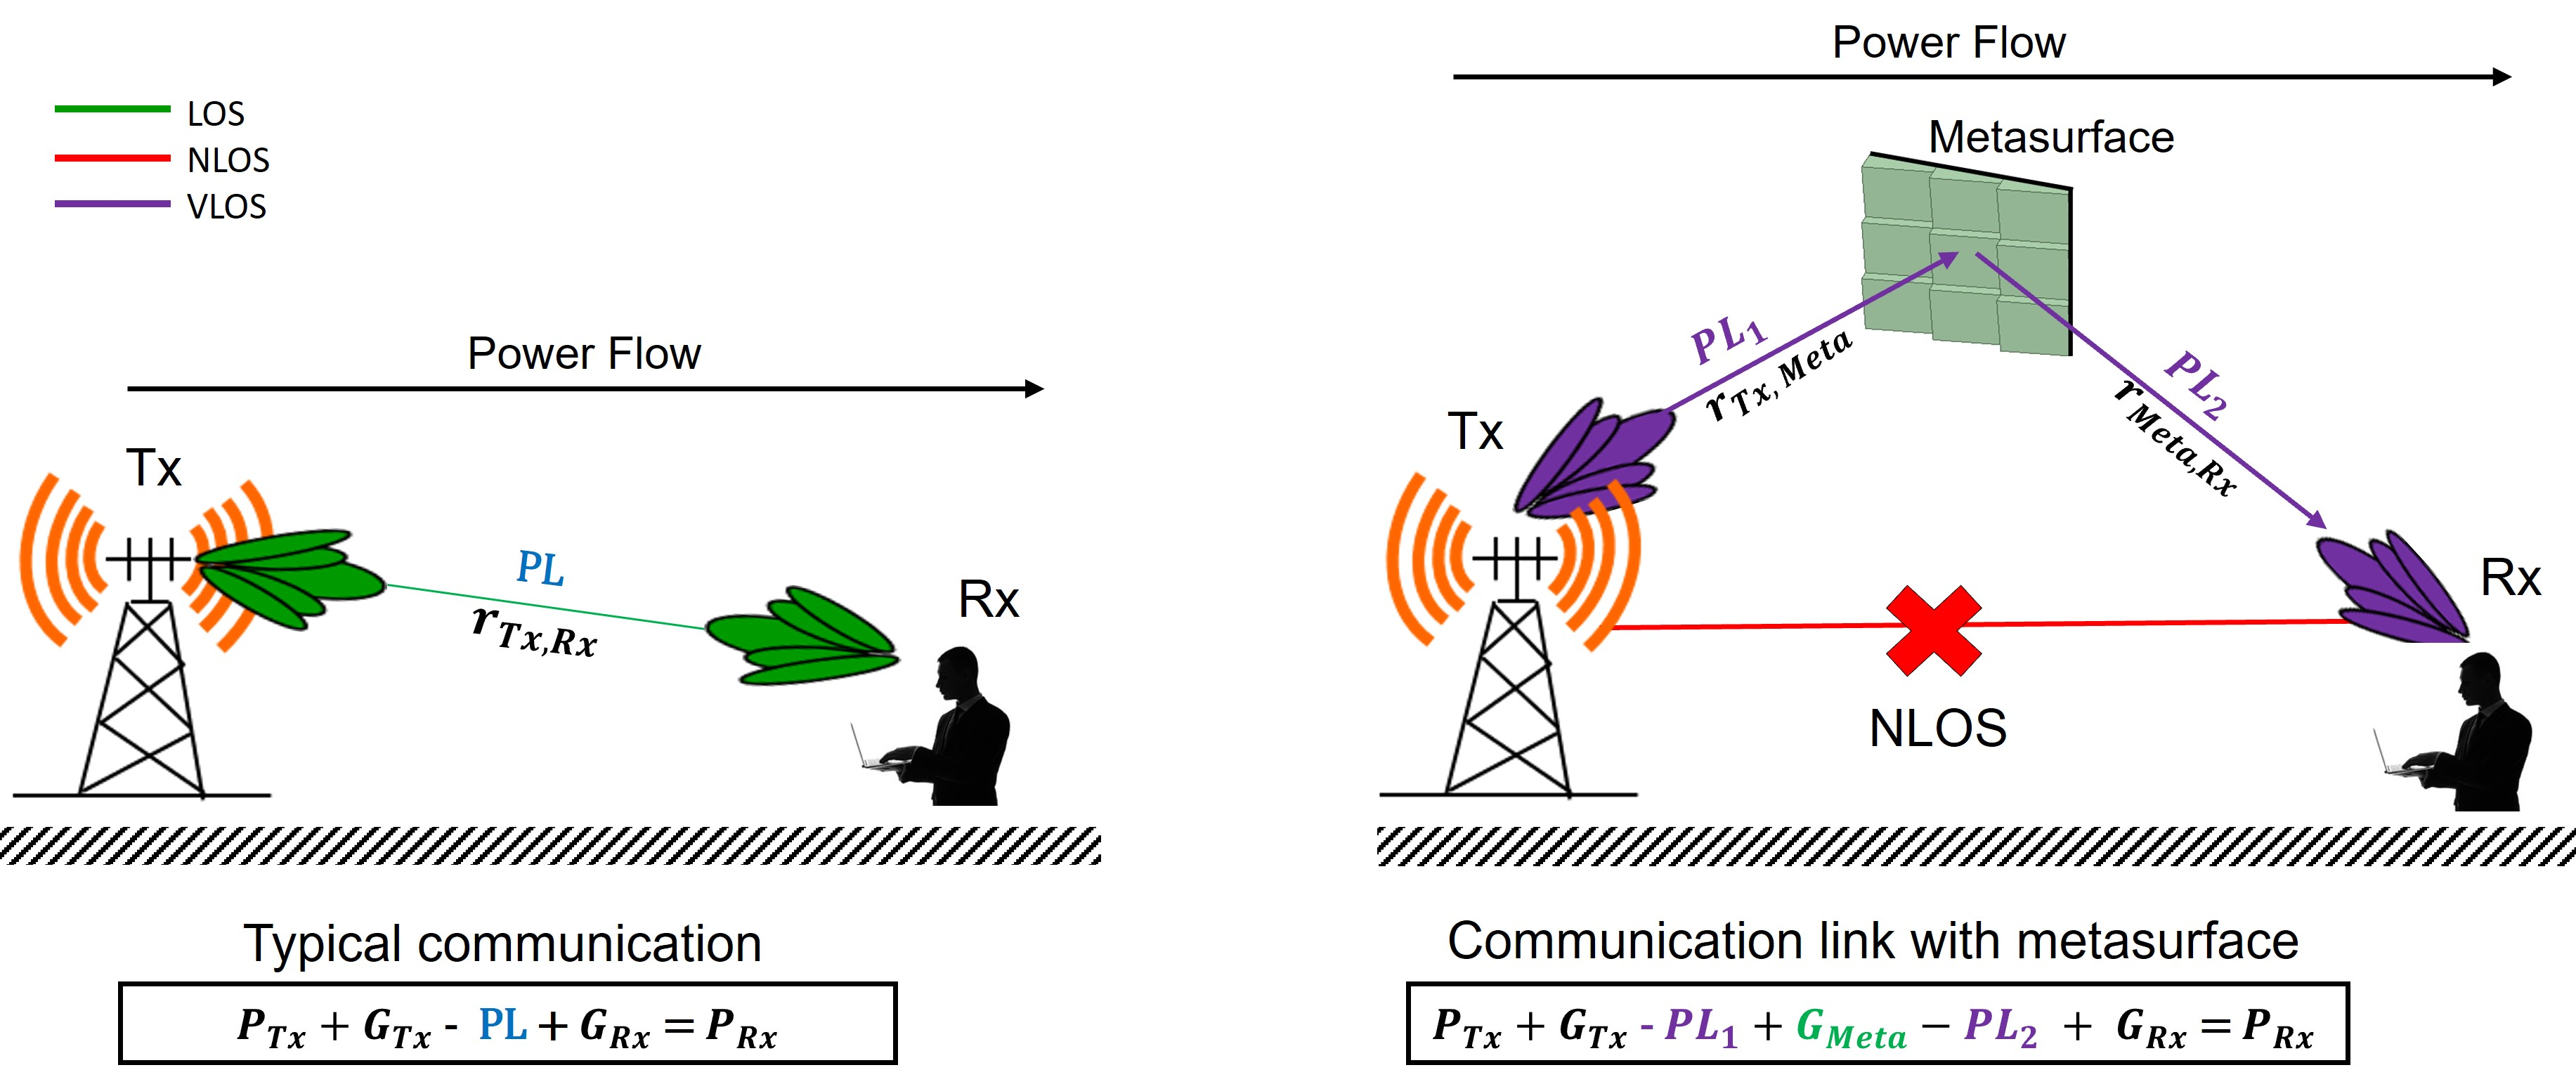
\includegraphics[width=0.9\linewidth]{images/Section 2 Images/Comm_link}
	\caption{Illustration of 6G downlink transmission without (left) and with metasurface (right). In this work, we are particularly interested in deploying IRSs to enable efficient communication in  NLOS regimes by using two LOS subchannels.}
	\label{fig:commlink}
\end{figure}
\Cref{fig:commlink} shows a comparison of the usual communication link without and with metasurface integration. The traditional communication link running from the transmitter to the receiver is depicted on the left side of the figure. The relationship established in this context is defined by classical parameters, i.e., $P_{Tx}$, $P_{Rx}$, $G_{Tx}$, $G_{Rx}$, and $PL$ between them. On the right of \Cref{fig:commlink}, we consider metasurfaces to serve NLOS users. The communication link is established between the transmitter to metasurfaces and, to the receiver. In addition to the classical parameters, we observe two subchannels i.e., Tx-metasurface, and metasurface-Rx, and introduce path losses between them which are given by $PL_{1}$ and $PL_{2}$, which is then compensated by the gain at the metasurfaces $G_{Meta}$.

\begin{figure}[tb]
	\centering
	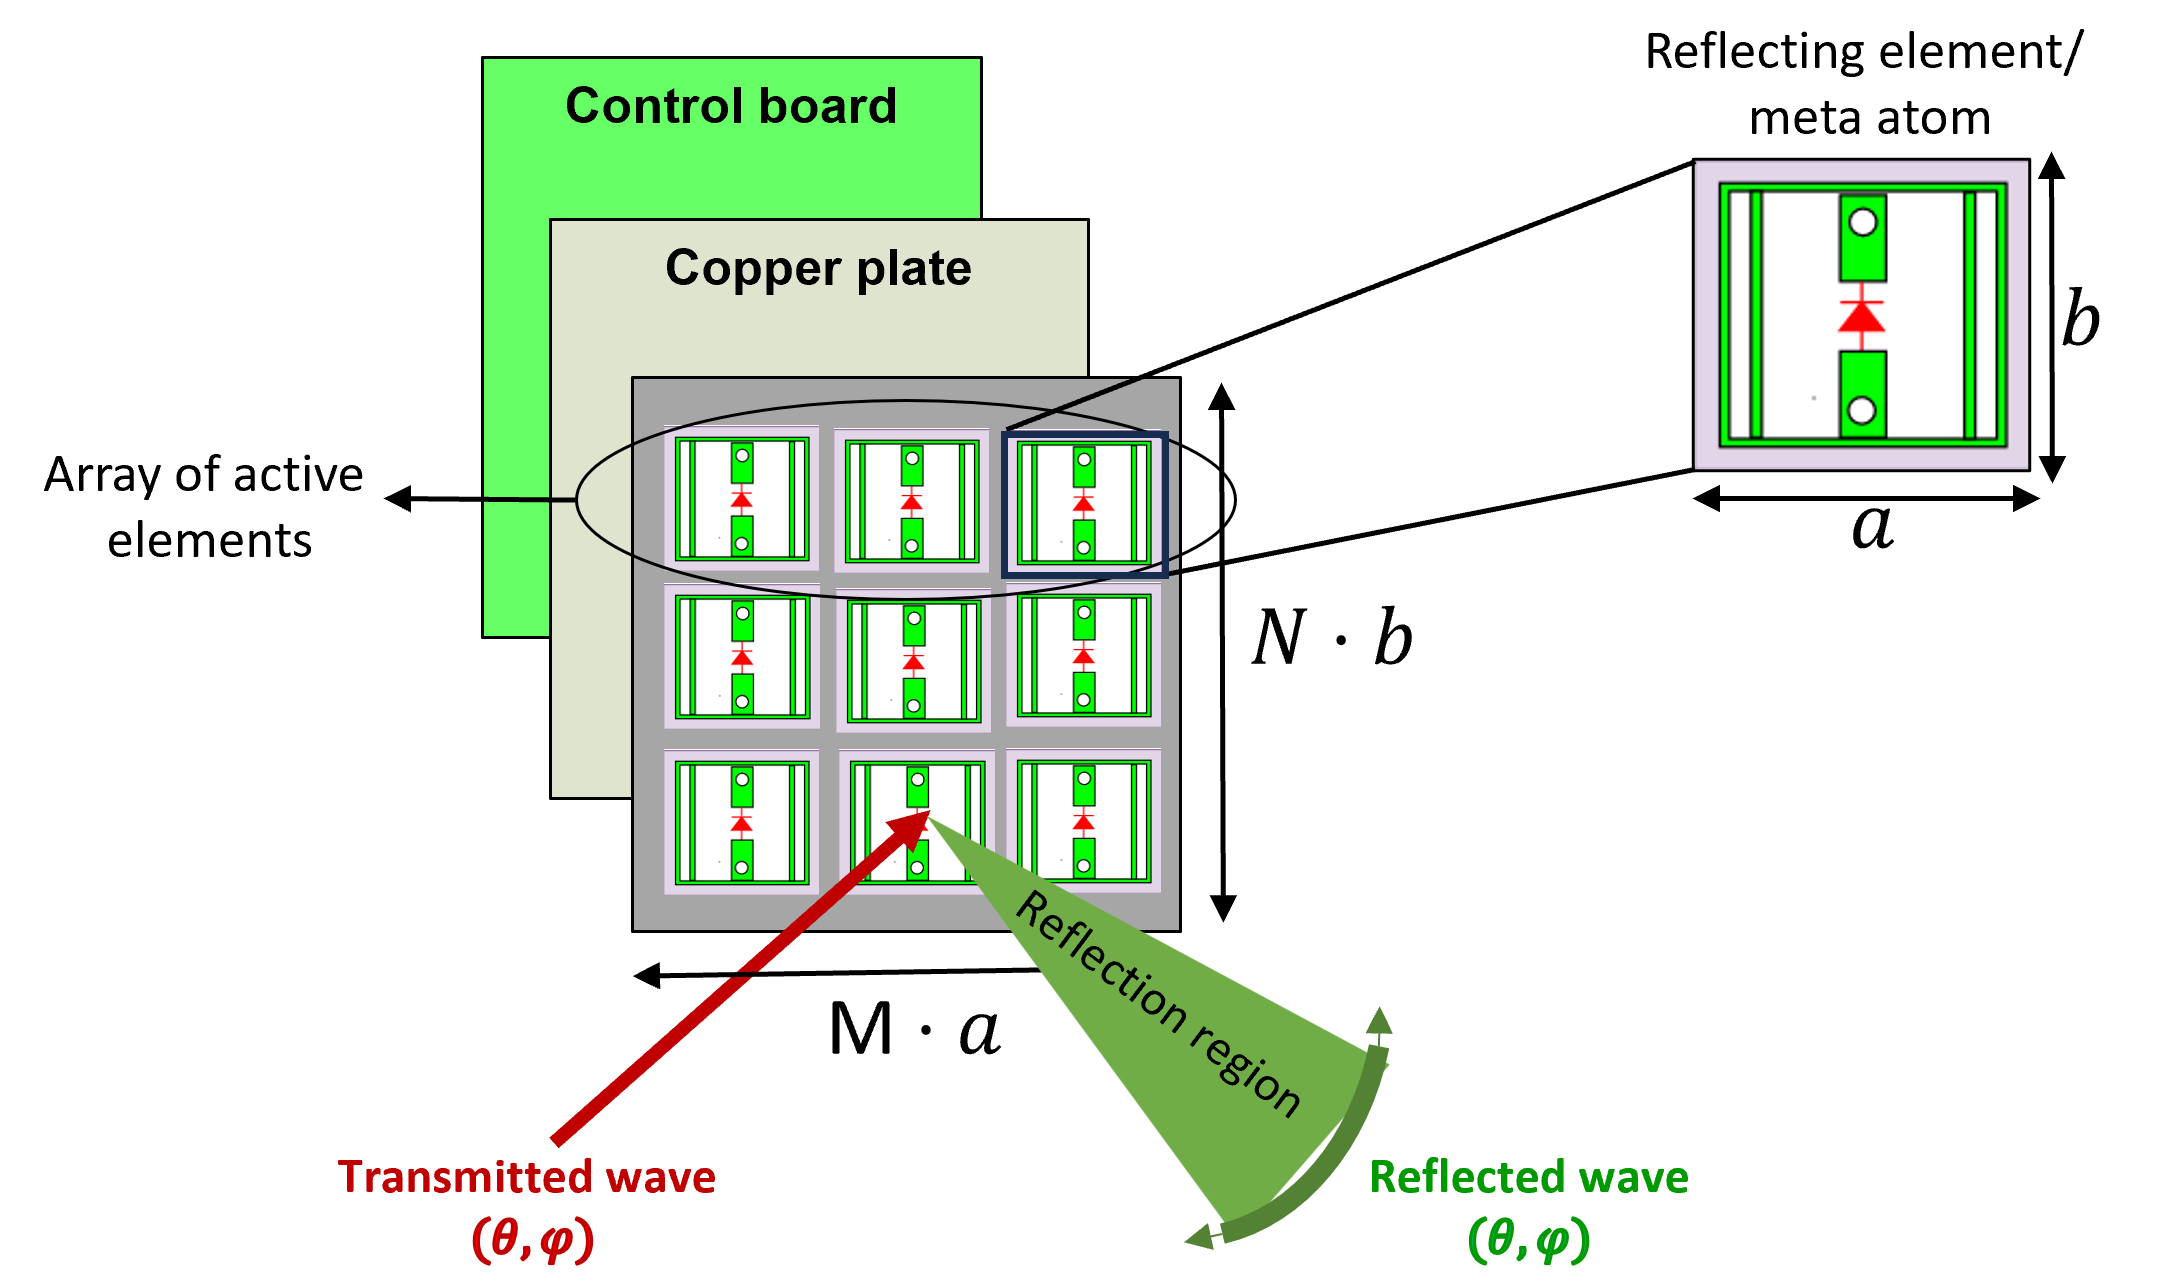
\includegraphics[width=1.0\linewidth]{images/Section 2 Images/IRS}
	\caption{Design and architecture of IRS with an array of active elements where the transmitted wave is reflected in a controllable manner in the reflection region for the overall dimensions of $(M\times a) \cdot (N \times b)$.}
	\label{fig:irs}
\end{figure}
\Cref{fig:irs} depicts the structural architecture of an IRS model. They are made up of sub-wavelength unit cells constituting a planar array of $M \times N$ active elements whose dimensions are $a \times b$, respectively. As mentioned previously, they can alter the interaction between the incident wave and the surface. We will examine two crucial of many feasible crucial metasurface features in more detail in the next sections. First, we consider IRSs in \Cref{IRS}, which may actively direct the reflection into the target direction with the reflection pattern being configured in real-time as desired, focusing on flexibility and adaptability to enhance the coverage and signal strength. Second, we discuss passive reflectors in \Cref{Passive reflectors}, which are entirely passive in nature, i.e., not reconfigurable, but still provide a customized reflection pattern with zero power consumption.

\subsection{Design and Architecture of Intelligent Reflecting Surfaces} \label{IRS}
\ac{IRS}s contain a variety of tiny, reconfigurable reflecting components, enabling precise shaping of the arising reflection pattern by modifying the phase and amplitude of the reflected waves. When compared to reflect-arrays, \ac{IRS}s are instead placed in the far-field regions of Tx and Rx, i.e., at practical positions such as building facades \cite{IRS_citations}.

The functionality of the \ac{IRS} depends heavily on its design and architecture which are created to be flexible, and scalable for a variety of wireless applications as shown in  \Cref{fig:irs}. An \ac{IRS} typically consists of a planar array of unit cells whose dimensions are $a \times b$. These may modify the characteristics of electromagnetic waves' phase, amplitude, and polarization \cite{wu2019towards}. The performance metrics depend on, e.g., the spacing density and number of control bits of the unit cells. These parameters, but also the IRS material affect the supported carrier frequency and bandwidth. Most important, however, is the setting of each unit cell, e.g., in terms of phase as the superposition of the individual unit cells' interactions with the incident EM wave yields the overall IRS performance. Determination of these settings is the main design factor for real-time operation \cite{IRSdesignandapp, Shen2020ModelingAA, wu2019towards}.

6G use cases for IRSs are, for example, as follows: To increase signal strength and coverage inside a building, for instance, one to several \ac{IRS}s can be mounted on available wall sections or the ceiling \cite{IRSdesignandapp}. This way, fewer antenna sites are required such that costs and power consumption are reduced. An \ac{IRS} can also be used to lessen interference to further enhance the quality of wireless communications. Other usage concepts envision improved security and privacy for wireless communications by, in essence, building a physical barrier that prevents signals from being intercepted or eavesdropped. 

Considering the active elements, IRSs need a power line or battery for continuous operation. Additionally, the IRS needs to be controlled by the network operator via a wired link or a wireless connection to the Tx. As an IRS numerous unit cells can form reflection beams similar to an antenna array forming pencil or sector beams, these configurations shall be provided by the network operator along the control link \cite{IRS_citations2}. For this purpose, however, novel signaling procedures similar to the beam management described in \Cref{Millimeter wave communication} is required for 6G.
\subsection{Passive Reflectors and the HELIOS Concept} \label{Passive reflectors}
However, there are some real-world difficulties with the \ac{IRS}, such as the need to deal with the complexity of hardware implementation, scalability, and rising energy consumption with size. While \ac{IRS} represents an evolution for future 6G communications in wireless communication, passive reflectors present a scalable, non-reconfigurable alternative feasible in the short term. In contrast to active IRSs, passive reflectors may not amplify signals but either bundle or scatter the incident energy into a predetermined and fixed direction. Passive reflectors can be created like the metasurfaces outlined in \Cref{IRS} \cite{LiSinghSievenpiper, FangLiChenSunXiaoHeZhou}, but without the use of adjustable unit cells. Alternative techniques, such as HELIOS \cite{Helios}, are also conceivable as explained below.
\subsubsection{Introduction of HELIOS Concept} \label{Introduction of HELIOS Concept}
In light of the previously discussed drawbacks of IRSs, passive reflectors have some advantages over \ac{IRS} in certain situations. The majority of passive reflectors posses typically fixed structures made up of strategically placed metallic surfaces or objects \cite{Anjinappa, Passiverefl}. Their position and geometry can be deliberately exploited to realize the desired reflection behavior as needed to optimize the communication performance. Naturally, their fixed position and shape make them compatible with existing wireless communication systems as there is no need for novel control links and signaling procedures, while also removing the need for a power supply. Thus, the advantage comes in the simplicity which is expected to also reduce costs. Moreover, passive reflectors are expected to be very dependable for tough outdoor settings coming with challenges regarding temperature (hot and cold), moisture, UV radiation, and wind.

Passive reflectors, in this work represented by the HELIOS \cite{Helios} concept, come with the above-described features and may quickly revolutionize the wireless network infrastructure landscape. The core approach is as follows:
\begin{itemize}
	\item Seamless, piecewise installation that easily merges into urban settings without imposing any power supply demands.
	\item Sleek design and manufacturing method not only meets network operators’
	rigorous criteria but also improves network coverage capabilities.
	\item The combination of passive reflectors with cutting-edge processes such as 3D printing and precise spray painting opens up new options for customization and adaptability.
\end{itemize}
\begin{figure}[tb]
	\centering
	\subfloat[$2 \times 2$ HELIOS reflector array with $a=\SI{10}{\centi\meter}$, $b=\SI{5}{\centi\meter}$, $\alpha_{m,n}=20^\circ$, and $\beta_{m,n}=10^\circ$.]{
		\includegraphics[width=0.3\linewidth]{images/Section 2 Images/model_2x2}
		\label{fig:model_2x2}
	}
		\hfill
	\subfloat[$4 \times 1$ HELIOS reflector array with $a=\SI{20}{\centi\meter}$, $b=\SI{10}{\centi\meter}$, $\beta_{m,n}=10^\circ$, and $\alpha_{1,1},\dots,\alpha_{4,1}=(5,10,15,20)^\circ$.]{
		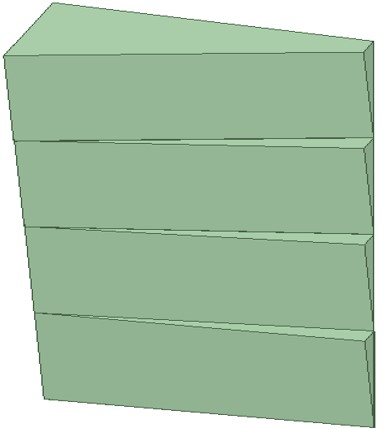
\includegraphics[width=0.3\textwidth]{images/Section 2 Images/model_4x1}
		\label{fig:model_4x1}
	}
		\hfill
	\subfloat[$8 \times 8$ HELIOS reflector array with $a=\SI{10}{\centi\meter}$, $b=\SI{15}{\centi\meter}$, $\alpha_{m,n}=10^\circ$, and $\beta_{m,n}=15^\circ$.]{
		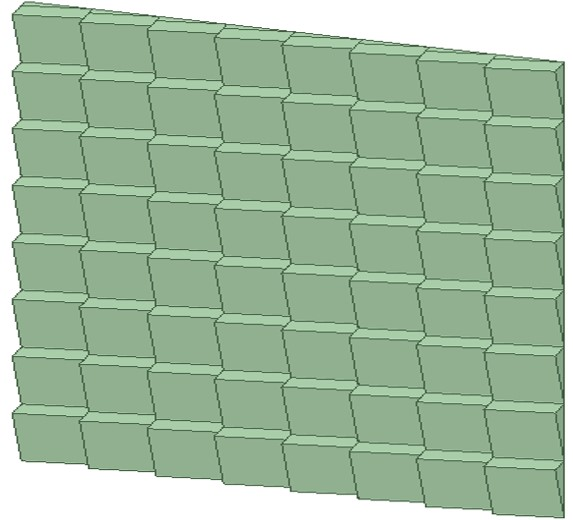
\includegraphics[width=0.3\textwidth]{images/Section 2 Images/model_8x8}
		\label{fig:model_8x8}
	}
	\caption[Illustration of HELIOS reflector arrays with different dimensions, sizes, and slope angles, showcasing the high degree of flexibility of the model.]{Illustration of HELIOS reflector arrays with different dimensions, sizes, and slope angles, showcasing the high degree of flexibility of the model.}
	\label{fig:model_array}
\end{figure}
We will now delve into the authors' design and production process for their HELIOS reflectors. The first step constitutes the careful selection of a suitable geometry, i.e., one with the capacity to successfully reflect the incident electromagnetic wave into the desired direction range. Another critical component of the geometry design is its unobtrusiveness, i.e., minimization of the exhibited protrusion for better technology acceptance \cite{Helios}. Following that, the authors choose suitable materials and production processes depending on the deployment scenario under aspects of durability, resource efficiency, and costs.

The HELIOS reflector array's adaptation to various configurations, which display a range of dimensions, reflector sizes, and slope angles, is a testament to its versatility as illustrated in \Cref{fig:model_array}. The versions that are shown have different values, which highlights the amazing adaptability that the design offers. Because of its adaptation to many settings, this variability highlights the model's versatility and enables customization depending on unique requirements, making it a highly flexible model.
\subsubsection{Construction of Geometry of HELIOS Reflector Module}
The primary principle controlling the geometry selection of the reflector is the application of Snell's law of reflection \cite{7728465}. When dealing with a flat reflecting plate with dimensions $a \times b$, our method involves an incident wave meeting the surface at azimuth and elevation angles, with the reflected wave preserving identical angles relative to the surface normal, cf. \Cref{fig:HELIOS1}. As we move into the domain of three-dimensional passive reflectors, the problem becomes custom-tailoring these structures to precisely focus the transmitted beam towards the specified receiver direction, by the criteria of our network planning.

To accomplish this, the authors designed a saw-tooth-like structure for the reflector, with the depth of each protrusion decreasing proportionally as the number of modules grows \cite{Helios}. \Cref{fig:HELIOS2}, and \Cref{fig:HELIOS3} illustrate the impact of an individual module's horizontal tilt angle $\alpha$ on the azimuth reflection angle $\varphi_{out}$ and, in addition, the joint case in which a vertical slope angle $\beta$ further affects the elevation reflection angle $\theta_{out}$. It is worth mentioning that the parametrization of the reflector
\begin{figure}[H]
	\centering
	\subfloat[Basic rectangular flat plate with no element of slope angles with the depiction of Snell's law of reflection.]{
		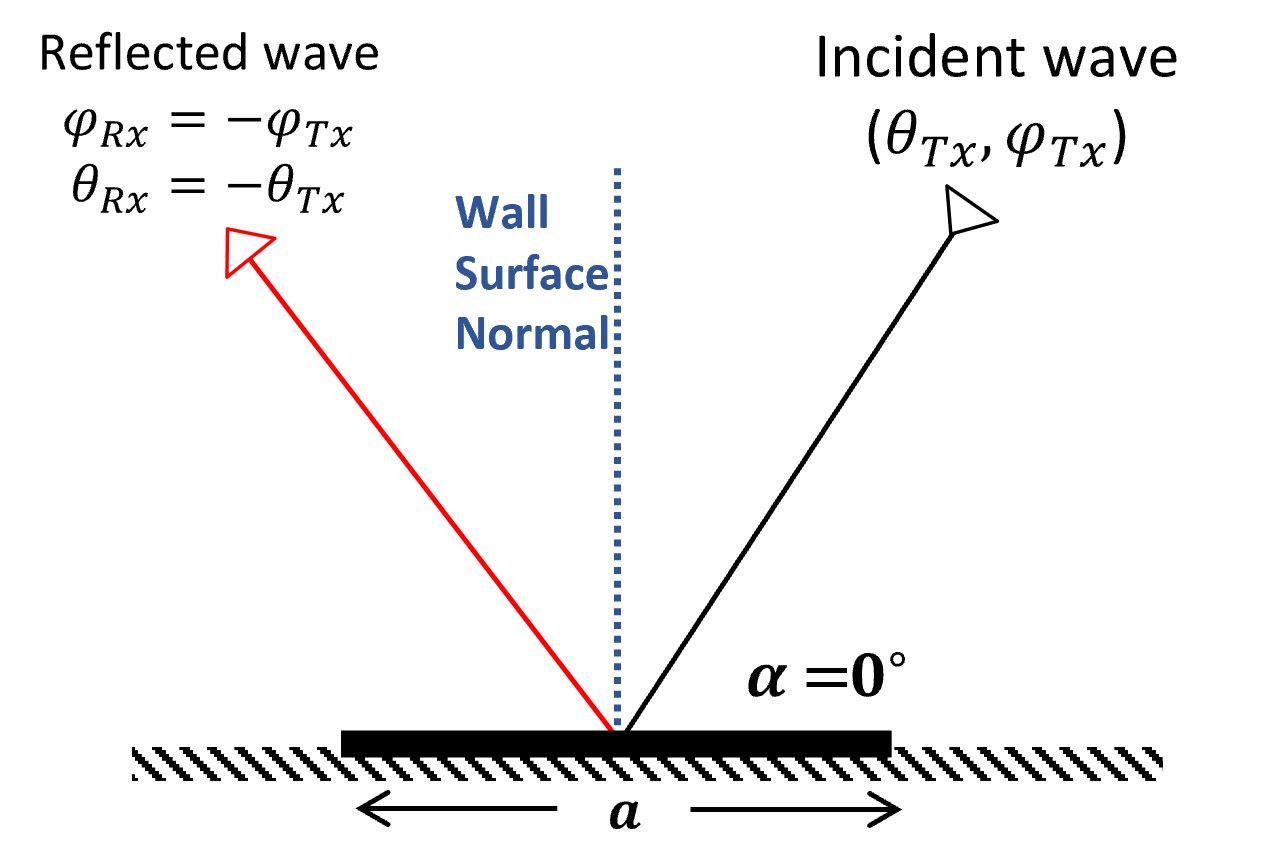
\includegraphics[width=0.3\linewidth]{images/Section 2 Images/HELIOS_1}
		\label{fig:HELIOS1}
	}
	\hfill
	\subfloat[HELIOS module with slope angle $\alpha$ with a height $h$, depicting the shift in the reflected wave by two times the $\varphi_{Tx}$.]{
		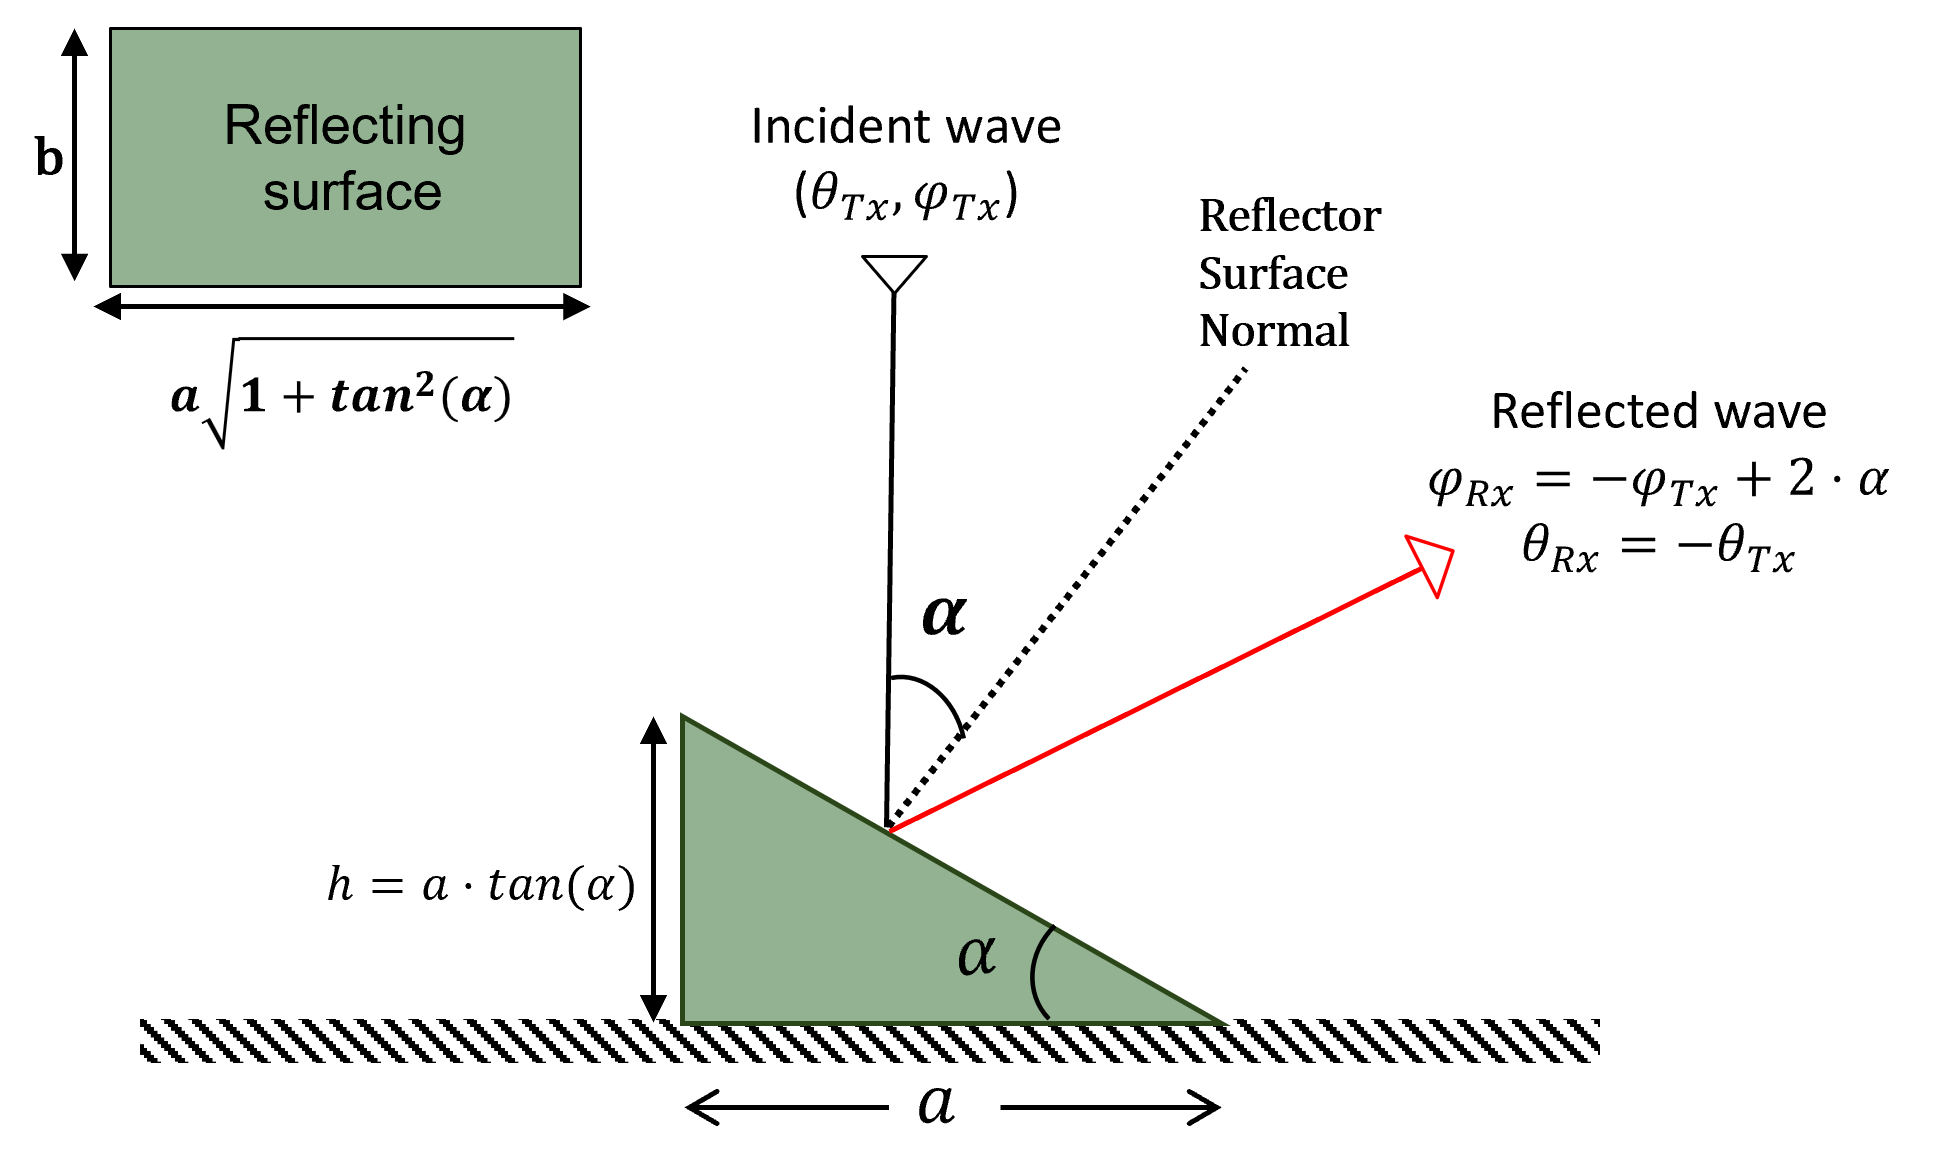
\includegraphics[width=0.3\textwidth]{images/Section 2 Images/HELIOS_2}
		\label{fig:HELIOS2}
	}
	\hfill
	\subfloat[HELIOS module with slope angle $\alpha$ and $\beta$ with a height $h$, depicting the shift in the reflected wave by two times the $\varphi_{Tx}$ and $\theta_{Tx}$.]{
		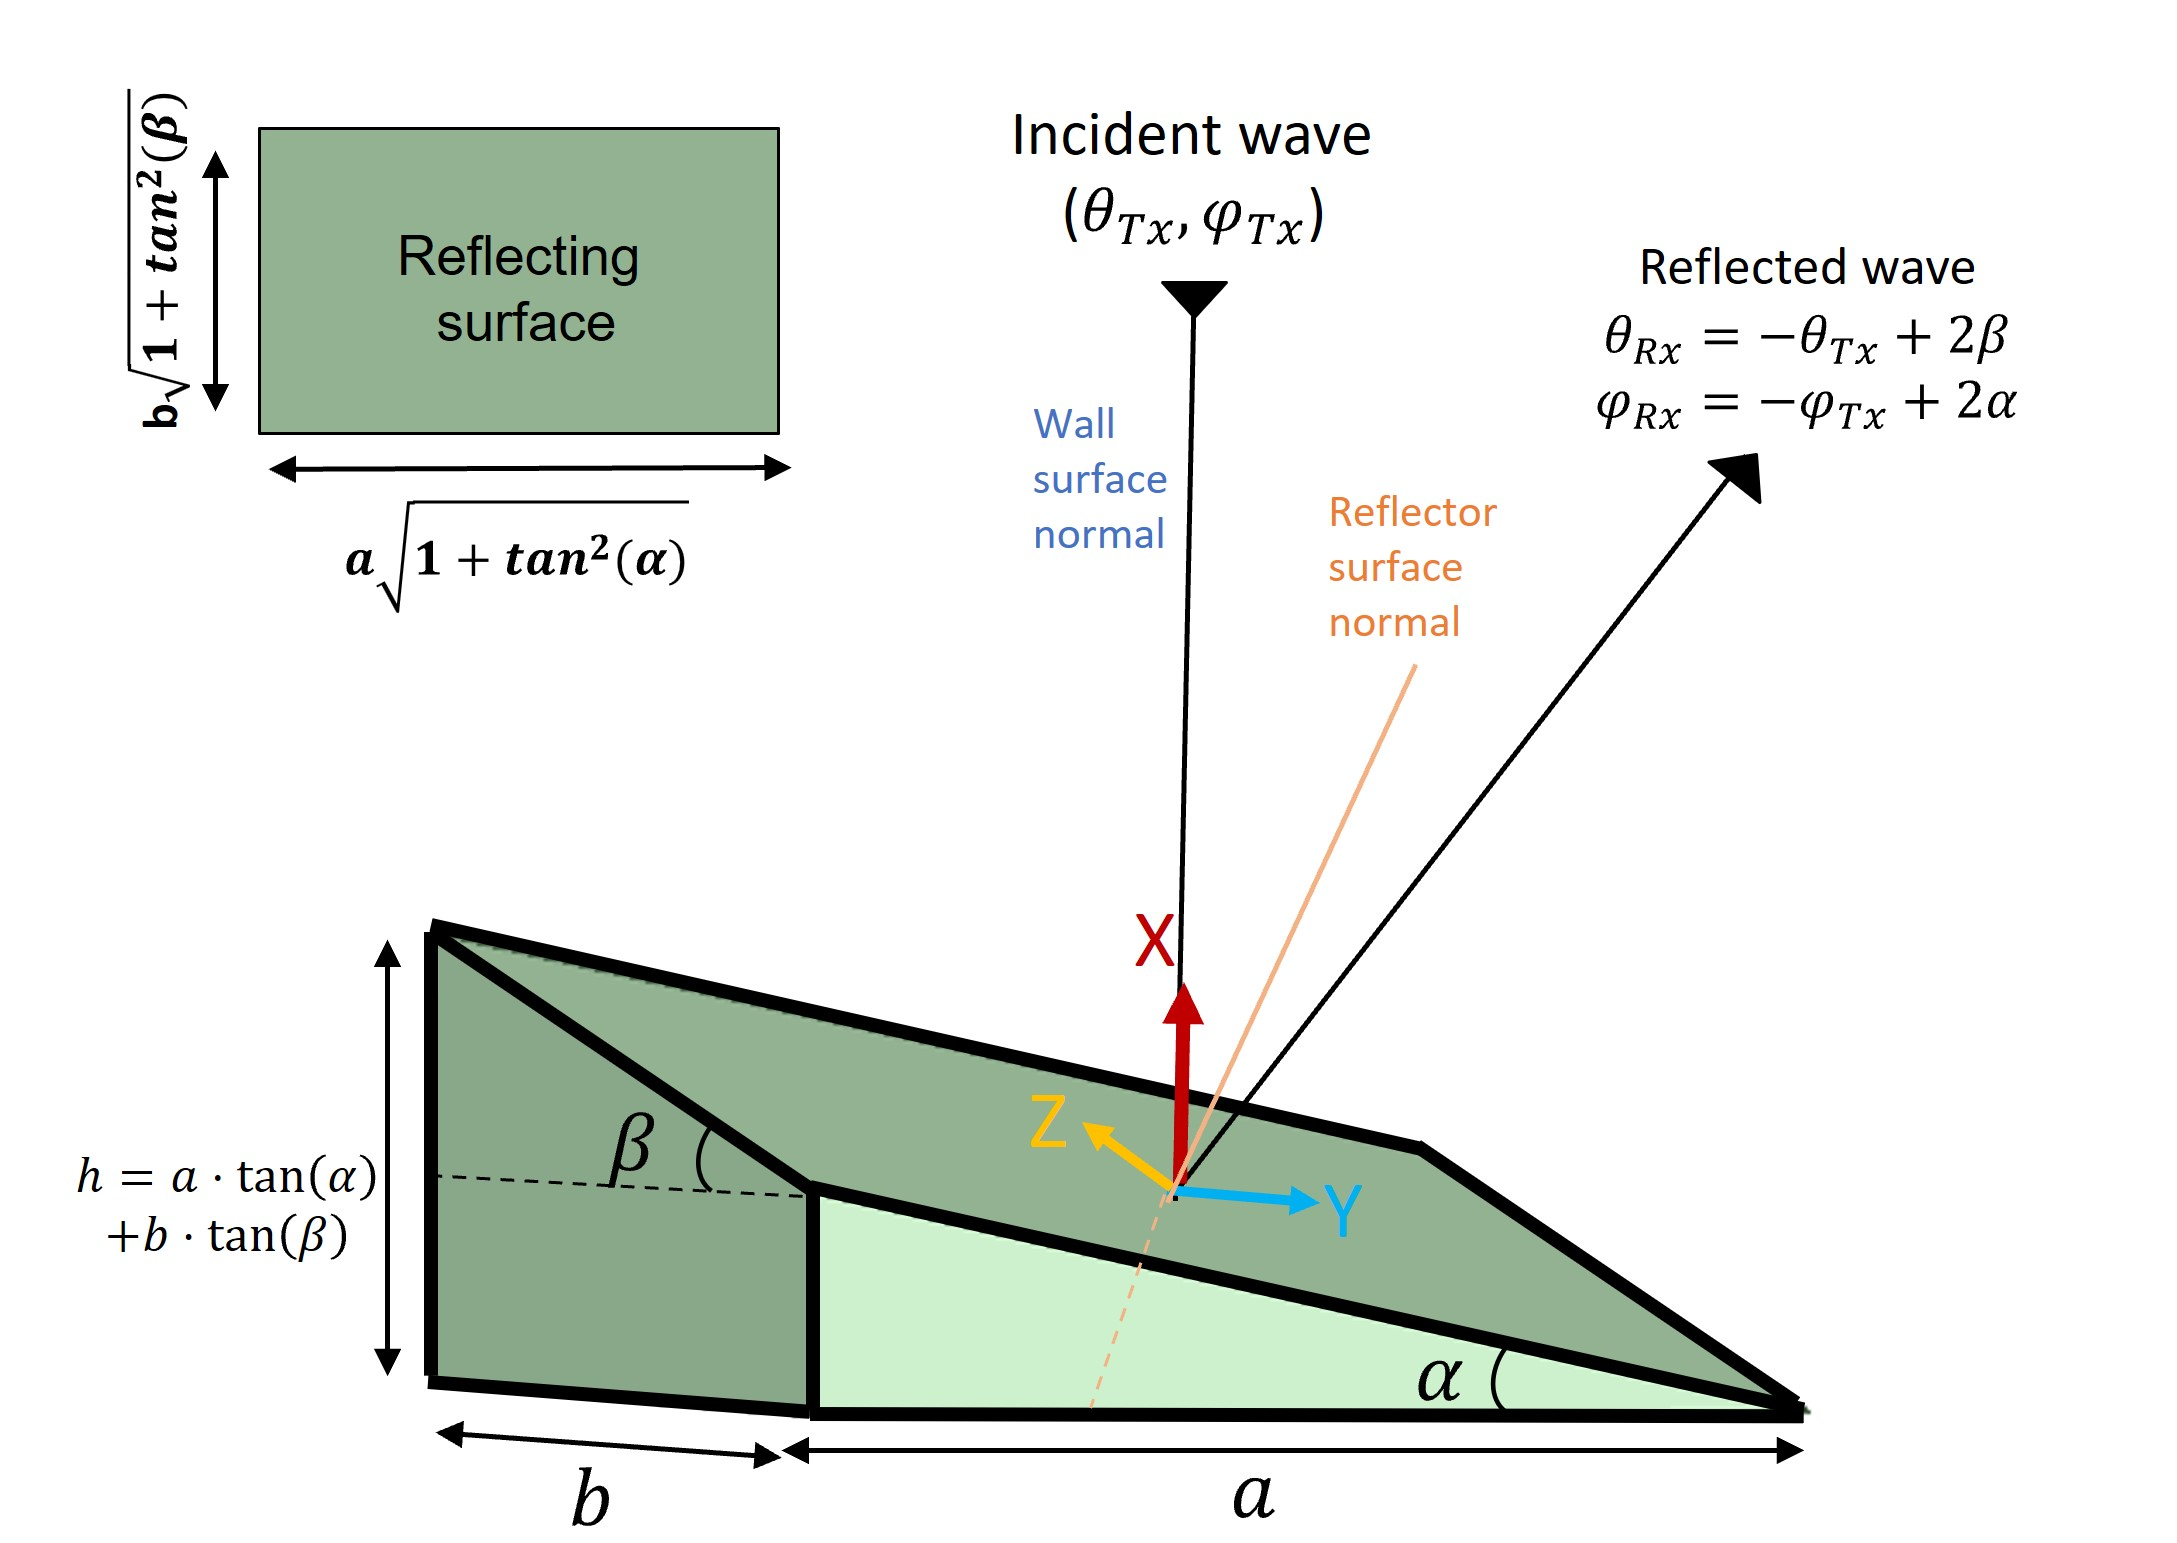
\includegraphics[width=0.32\textwidth]{images/Section 2 Images/HELIOS_3}
		\label{fig:HELIOS3}
	}
	\caption[Horizontal and vertical tilting of the reflecting surface enables deliberate steering of the reflection towards the desired direction.]{Horizontal and vertical tilting of the reflecting surface enables deliberate steering of the reflection towards the desired direction. }
	\label{fig:tricdvsuq}
\end{figure}
module, which includes variables such as vertical and horizontal slope angles namely $\alpha_{m,n}$ and $\beta_{m,n}$, reflector element base size $a \times b$, and indices $m \in 1, \dots, M$ and $n \in 1, \dots, N$ with $M \times N$ specifying the number of HELIOS modules.
\subsubsection{Material Selection}
Reflectors are often made of highly conductive materials to minimize signal loss. While traditional options such as solid metal reflectors or aluminum foil are effective, they come with high material prices \cite{Helios}. Moreover, reshaping supplies of metal into the desired HELIOS form may complicate production, and thus, increase costs. The HELIOS concept addresses these issues as follows. Using 3D printing with a suitable filament, e.g., PLA for indoor deployments, arbitrary shapes may be produced. Afterward, a conductive coating is given via spray-coating.
\subsection{Common Coordinate System and Parameters for Metasurface Characterization} \label{coordinate systems}
The investigation of metasurfaces for \ac{mmWave} communication leverages the subsequently described cartesian reference coordinate system, as illustrated in  \Cref{fig:3D model}. A 3D space defined by the three perpendicular axes ($x,y$, and $z$) in this coordinate system, which enables us to precisely find and describe the position and orientation of components in wireless communication systems. For example, the reflecting surface shall be in the $y$-$z$-plane.

Let us consider a planar EM wave impinging on the reflecting surface. The direction of this wave is indicated by its wave vector $\overrightarrow{\textbf{k}}$ which can be related to the direction of the normal vector $\overrightarrow{\textbf{n}}$ of the surface \footnote{Note that vector n has a positive z-component, otherwise, the vector would point into the building or ceiling at which the reflector is mounted.}. As depicted by  \Cref{Vectork} vectors $\overrightarrow{\textbf{k}}$ and $\overrightarrow{\textbf{n}}$ can be described relative to the reflecting surface using spherical coordinates, namely azimuth angle $\varphi_k \in [-180:180]^\circ$ (defined in $y$-$z$-plane from $y$-axis in the direction of $z$-axis) and elevation angle $\theta_k \in [-90:90]^\circ$ (defined in $y$-$z$-plane towards $x$-axis), as well as the magnitudes $n$=\num{1} and $k= \frac{2 \cdot \pi}{\lambda}$.
\begin{equation} \label{Vectork}
	\begin{split}
		\overrightarrow{\textbf{k}} &= (k, \theta_{k}, \varphi_{k})\\
		\overrightarrow{\textbf{n}} &= [1, 0, 0]
	\end{split}
\end{equation}
Using the described parameters, we describe vector $\overrightarrow{\textbf{k}}$ in Cartesian coordinates as follows:
\begin{figure}[tb]
	\centering
	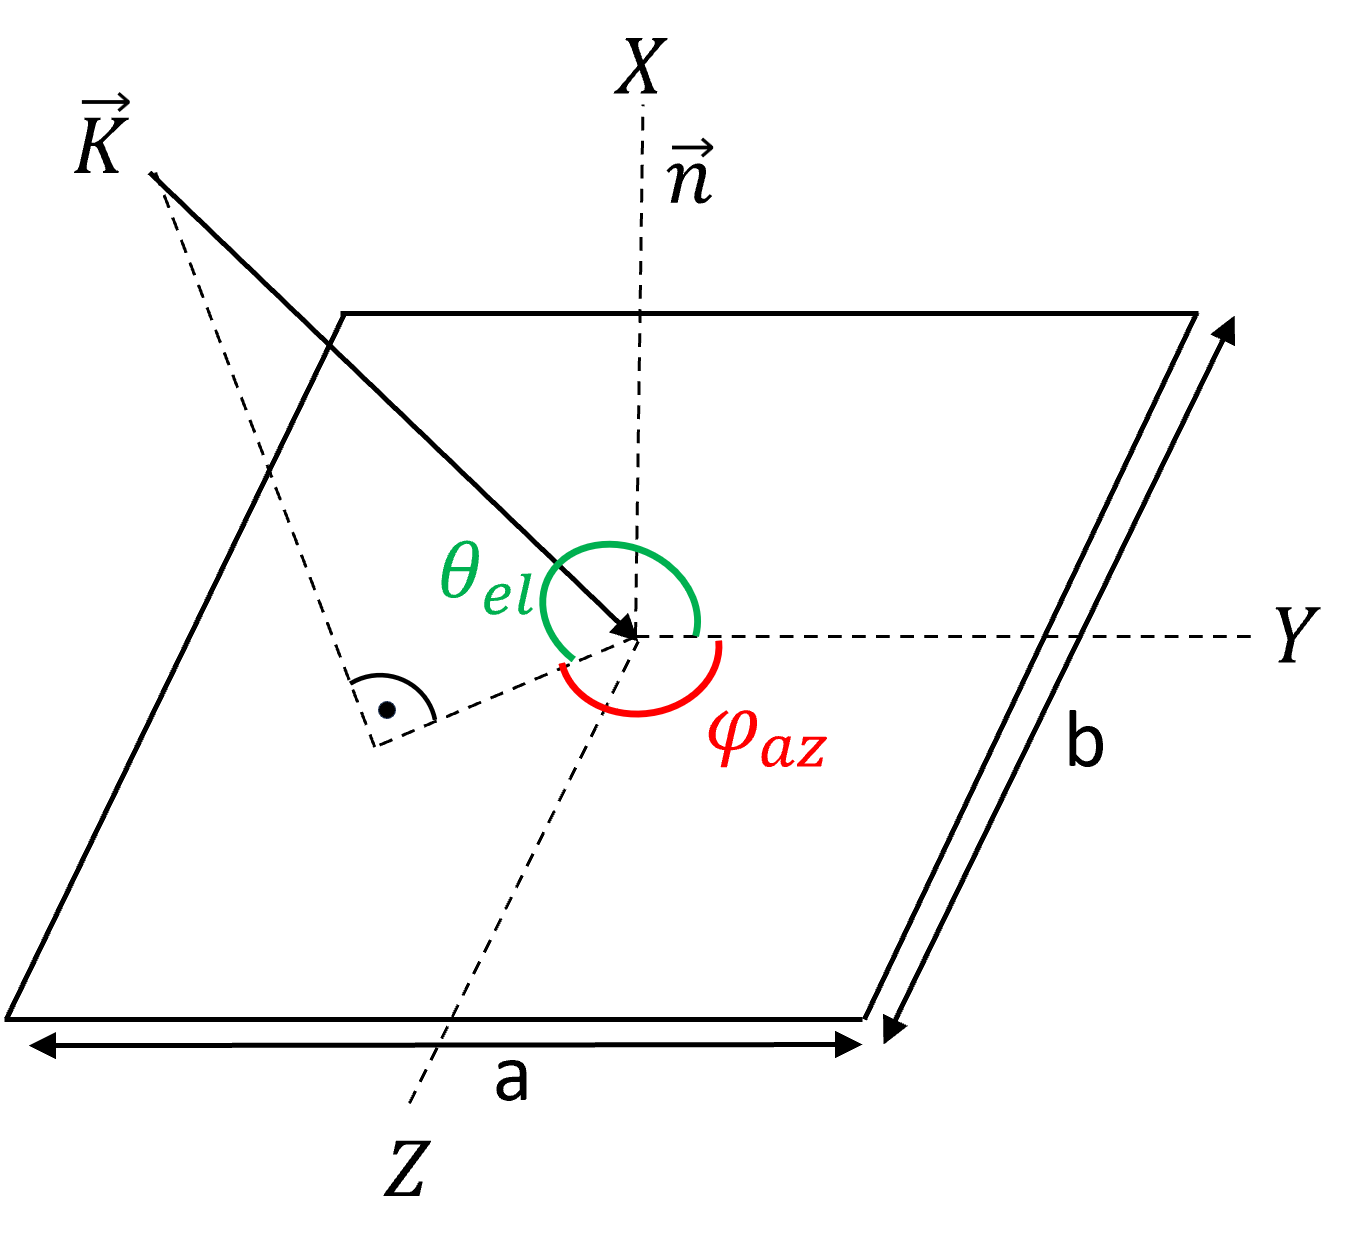
\includegraphics[width=0.5\linewidth]{images/Section 2 Images/coordinate_system}
	\caption{Plane wave impinges along direction k on reflecting surface in $y$-$z$-plane with elevation angle $\theta_{el}$ and azimuth angle $\varphi_{az}$ in \si{\deg}.}
	\label{fig:3D model}
\end{figure}
\begin{equation} \label{Eq:Coordinates conversion of impinging wave vector_1}
	\overrightarrow{\textbf{K}} =
	\begin{bmatrix}
		k_x\\ k_y\\k_z
	\end{bmatrix}
	= k
	\begin{bmatrix}
		\cos(\theta_{k}) \cdot  \cos(\varphi_{k})  \\ 
		\cos(\theta_{k}) \cdot \sin(\varphi_{k})\\
		\sin(\theta_{k})
	\end{bmatrix}
\end{equation}
Furthermore, we may deduce the spherical coordinate system parameters from the Cartesian description as follows:
\begin{equation} \label{Eq:theta_inc and varphi_inc}
	\begin{split}
		\theta_{k} &= \arccos{\frac{k_z}{|\overrightarrow{\textbf{k}}|}} \\
		\varphi_{k} &= \arctan{\frac{k_y}{k_x}} 
	\end{split}
\end{equation}
where $|\overrightarrow{\textbf{k}}|$ is the magnitude of impinging wave vector $\overrightarrow{\textbf{k}}$.
\begin{equation}
	|\overrightarrow{\textbf{K}}|= k= \sqrt{k_x^2+ k_y^2+ k_z^2}
\end{equation}
In the following, we will refer to the incident  wave vector using $\overrightarrow{\textbf{K}_{Tx}}$, whereas the reflected wave uses $\overrightarrow{\textbf{K}_{Rx}}$. Based on the law of reflection, the angle of the incident is implicitly defined by the reflection angle, given by \Cref{Eq:law of reflection}. So, the elevation and azimuth angles of the impinging and reflecting waves will have the same magnitude but different signs.
\begin{equation} \label{Eq:law of reflection}
	\begin{split}
		\theta_{Rx} &= -\theta_{Tx}\\
		\varphi_{Rx} &=  -\varphi_{Tx}
	\end{split}
\end{equation}
Let us consider the Euclidean norm angles to be $\gamma_{Tx}$ and $\gamma_{Rx}$ at the transmitter and the receiver, respectively. As defined in  \Cref{Eq:euclidean norm}, they define the overall deviation angle from the $x$-axis.
\begin{equation} \label{Eq:euclidean norm}
	\begin{split}
		\gamma_{Tx} &= \sqrt{\theta_{Tx}^2+\varphi_{Tx}^2}\\
		\gamma_{Rx} &= \sqrt{\theta_{Rx}^2+\varphi_{Rx}^2}
	\end{split}
\end{equation}
In the following sections, the previous metasurface geometry relations will be applied. \Cref{Variable abbreviation} extends these with additional parameters incorporating the above geometry into a wide communication system description including the Tx and Rx.
\begin{table}[H] % H -> dieses objekt wird genau da wo der code steht festgenagelt
	\footnotesize
	\caption{Comprehensive standardization of parameters: Units and abbreviations for metasurface channel modeling across the entire thesis.}
	\label{Variable abbreviation}
	\centering
	\begin{tabular}{C{3cm}|C{7cm}|C{2.5cm}}
		\textbf{Abbreviation} & \bf Definition & \bf Units\\
		\hline 
		$\eta$ & Characteristic impedance & $\Omega$\\
		\hline 
		$f$ & Frequency & \si{\hertz} \\
		\hline 
		$c$ & Speed of light & \si{\meter}/\si{\second} \\
		\hline
		$\Gamma$ & Reflection coefficient & Unitless\\
		\hline 
		$k$ & Wave number & \si{\per\meter}\\
		\hline
		$\lambda$ & Wavelength & \si{\meter}\\
		\hline 
		$a$  & $y$-axis dimension of the \ac{IRS} & \si{\meter} \\
		\hline 
		$b$  & $z$-axis dimension of the \ac{IRS} & \si{\meter} \\
		\hline 
		$M$  & Reflector array on the $z$-axis of the \ac{IRS} & Unitless \\
		\hline 
		$N$  & Reflector array on the $y$-axis of the \ac{IRS} & Unitless \\
		\hline 
		$A_{eff}$ & Effective aperture of the \ac{IRS}  & $\si{\meter}^2$\\
		\hline 
		$ E_{incident}$  & Electric field strength of the incident signal & $V/\si{\meter}$\\
		\hline 
		$ E_{reflect}$  & Electric field strength of the reflected signal & $V/\si{\meter}$\\
		\hline 
		$P_{incident}$ & Power of incident signal & $W$ \\
		\hline 
		$ P_{captured}$ & Power captured by \ac{IRS} element & $W$  \\
		\hline 
		$ P_{reflected}$ & Power reflected by \ac{IRS} element & $W$  \\
		\hline 
		$P_{Rx}$ & Power received by the receiver & $W$ \\
		\hline 
		$ P_{Tx} $  & Transmit power & $W$ \\
		\hline 
		$G_{Tx} $ & Gain of transmit antenna & Unitless\\
		\hline 
		$G_{Rx} $ & Gain of receiver antenna & Unitless\\
		\hline
		$G_{IRS}$ & Gain of \ac{IRS} & Unitless \\
		\hline 
		$r_{Tx,Rx}$ & Distance from transmitter to receiver & \si{\meter}\\
		\hline 
		$r_{Tx,IRS}$ & Distance from transmitter to \ac{IRS} element & \si{\meter}\\
		\hline 
		$r_{IRS,Rx}$ & Distance from receiver to \ac{IRS} element & \si{\meter} \\
		\hline 
		$\theta_{Tx}$ & Elevation angle to the transmitter & \si{\deg}\\
		\hline 
		$\varphi_{Tx} $  & Azimuth angle to the transmitter & \si{\deg} \\
		\hline 
		$\theta_{Rx}$ & Elevation angle to the receiver & \si{\deg}\\
		\hline 
		$\varphi_{Rx} $  & Azimuth angle to the receiver & \si{\deg} \\
		\hline 
		$\theta_{dev}$ & Deviated elevation angle at the receiver & \si{\deg}\\
		\hline 
		$\phi_{dev} $  & Deviated azimuth angle at the receiver & \si{\deg} \\
		\hline 
		$\Phi_{IRS} $  & Phase shift by IRS unit cell & \si{\deg} \\
		\hline 
		$\gamma_{Tx}$ & Overall IRS angle of incidence & \si{\deg}\\
		\hline 
		$\gamma_{Rx} $  & Overall IRS angle of reflection & \si{\deg}\\
		\hline 
		$PL$ & Path loss & Unitless\\ 
		\hline
		$SNR$ & Signal-to-Noise ratio & Unitless\\
		\hline
		$\alpha$ & Elevation slope angle & \si{\deg}\\
		\hline 
		$\beta$ & Azimuth slope angle & \si{\deg}\\
		\hline 
		$Gain_{RCS} $ & Analytical gain at the reflector & \si{\decibel} \\
		\hline 
		$Gain_{Sim} $ & Simulated gain at the reflector & \si{\decibel}\\
	\end{tabular}
\end{table}
Now that we have a firm grasp of the coordinate system and the variables that will direct our study, we introduce three IRS channel models from the literature and examine each individually.
\subsubsection{Model by Özdogan \emph{et al}. (2020) \cite{8936989}} \label{Model 1}
For an \ac{IRS} that is set up to reflect an incoming wave from a far-field source in a beamforming like manner towards a far-field receiver in direction $\theta_{Rx}$, the authors in \cite{8936989} have used the physical optics approach to derive an end-to-end path loss expression. The model consists of a plate in the $x$-$y$-plane with dimensions $a \times b$ which is perfectly conducting. It is radiated upon with a linearly polarized EM wave at distance $r_{Tx, IRS}$ at angle $\theta_{Tx}$ between incident wave vector and $\overrightarrow{e_z}$, with $\theta_{Tx} \in [0, \frac{\pi}{2}] $. The whole setup can be seen in  \Cref{fig:model1}. In the following we briefly summarize the key results of the work in the form of two lemmas yielding equations that will be used in the scope of this thesis.

Due to its far-field nature, the impinging wave vector is a nearly plane wave and the distribution of the \ac{EM} fields for the incident plane wave is given by  \Cref{Eq:model1 EM_inc} where $\eta$ is the characteristic impedance of the medium.
\begin{equation} \label{Eq:model1 EM_inc}
	\begin{aligned}
		\overrightarrow{E}_{incident} &= E_{incident} \cdot e^{-j \cdot k \left( \sin{\theta_{Tx}} \cdot y - \cos{\theta_{Tx}} \cdot z \right) } {\overrightarrow{e_x}} \\
		\overrightarrow{H}_{incident} &= - \frac{E_{incident}}{\eta} \left( \cos{\theta_{Tx}} \cdot {\overrightarrow{e_y}} +\sin{\theta_{Tx}} \cdot {\overrightarrow{e_z}} \right) \cdot e^{-j \cdot k \left( \sin{\theta_{Tx}} \cdot y - \cos{\theta_{Tx}} \cdot z \right)}
	\end{aligned}
\end{equation}
The E-field will cause the plate's electrons to move and it'll only be in the $\overrightarrow{e_x}$ direction as they are orthogonal. A scattered wave is created as a result of the \ac{EM} radiation that the moving electrons produce.
\begin{figure}[H] % h -> dieses object wird grob in der nähe seines quelltextes erscheinen
	\centering
	\vspace{12pt} %% 12pt abstand zwischen text und grafik
	\includegraphics*[width=0.6\textwidth]{images/Section 2 Images/model1}
	\caption{Illustrating the setup of the IRS model with the 3D angles for the transmitted and reflected wave \cite{8936989}.}
	\label{fig:model1} 
\end{figure}

\textbf{Lemma 1}: Measured against $\overrightarrow{e_z}$, the squared magnitude of the scattered field in the $\overrightarrow{e_y}$, $\overrightarrow{e_z}$ plane, and at any observation angle $\theta_{Dev} \in [0, \frac{\pi}{2}]$ is given by \Cref{Eq:model1 lemma1}.
\begin{equation} \label{Eq:model1 lemma1}
	S(r_{IRS, Rx},\theta_{Dev}) = \left( \frac{a \cdot b}{\lambda} \right)^2 \frac{E_{incident}^2}{r_{IRS, Rx}^2} \cos^2\theta_{Tx} \left[ \sinc \left( \frac{\pi \cdot b}{\lambda}(\sin\theta_{Dev}-\sin\theta_{Tx}) \right) \right]^2
\end{equation}
at a far-field observation distance $r_{IRS, Rx} \geq \frac{2 \cdot max \left( a^2, b^2 \right) }{\lambda}$  \cite{8936989}.

\Cref{Eq:model1 lemma1} has several intuitive properties. For instance, the reflected power is proportional to the squared IRS surface area, i.e., $(a \cdot b)^2$. According to Snell's law, the maximum is attained if the argument of $\sinc=0^\circ$. For $\theta_{Dev} =\theta_{Tx}=0^\circ$ the reflection power is maximized, i.e., an IRS will be most beneficial the more the incident and reflected waves are perpendicular to the surface.

The angles $\theta_{Tx}$ and $\theta_{Dev}$ from earlier represent the ideal case, but the main goal of \ac{IRS} is to achieve total anomalous reflection, with its main beam pointing in the desired direction $\theta_{Rx}$. In order to obtain the ideal field distributions  $\overrightarrow{E}_{reflect}$ and $\overrightarrow{H}_{reflect}$ of the reflected or scattered wave, the surface must be created to divert the incident plane wave as given by  \Cref{Eq:model1 reflect EM}.
\begin{equation} \label{Eq:model1 reflect EM}
	\begin{aligned}
		\overrightarrow{E}_{reflect} &= E_{reflect} e^{-j \cdot k \left( \sin{\theta_{Rx}} \cdot y - \cos{\theta_{Rx}} \cdot z \right) } {\overrightarrow{e_x}}  \\
		\overrightarrow{H}_{reflect} &= - \frac{E_{reflect}}{\eta} \left( \cos{\theta_{Rx}} \cdot {\overrightarrow{e_z}} +\sin{\theta_{Rx}} \cdot {\overrightarrow{e_z}} \right) e^{-j \cdot k \left( \sin{\theta_{Rx}} \cdot y - \cos{\theta_{Rx}} \cdot z \right) }
	\end{aligned}
\end{equation}
\textbf{Lemma 2}: The squared magnitude of the scattered field in \Cref{Eq:model1 squared magnitude of the scattered field} at an arbitrary observation angle $\theta_{Dev} \in [-\frac{\pi}{2}, \frac{\pi}{2}]$ is when using an \ac{IRS} to reflect a signal in the desired direction $\theta_{Rx}$.
\begin{equation} \label{Eq:model1 squared magnitude of the scattered field}
	S(r_{IRS, Rx},\theta_{Dev},E_{incident}) = \left( \frac{a \cdot b}{\lambda} \right)^2 \frac{E_{incident}^2  \cdot \cos^2 (\theta_{Tx})}{r_{IRS, Rx}^2}  \left[ \\sinc \left( \frac{\pi \cdot b}{\lambda} \left(\sin\theta_{Dev}-\sin\theta_{Rx} \right) \right) \right]^2
\end{equation}
The maximum of  \Cref{Eq:model1 squared magnitude of the scattered field} is achieved when $\theta_{Rx}=\theta_{Dev} $, thus confirming that the IRS's reflection is maximized in the desired direction although power is also radiated with varying intensity into other directions. Therefore, this equation includes an important description of the IRS reflection pattern. Notably, it generalizes the hull curve described in \Cref{Eq:model1 lemma1}. With transmitter gain $G_{Tx}$ and receiver gain $G_{Rx}$, \Cref{Eq:model1 E and P } gives the relationship between $E_{incident}$ and transmit power $P_{Tx}$.
\begin{equation} \label{Eq:model1 E and P }
	\frac{E_{incident}^2}{2 \eta} = \frac{P_{Tx} \cdot G_{Tx}}{4 \cdot \pi \cdot r_{Tx,IRS}^2}     
\end{equation}
The effective area $A_{eff} $ of the receiver antenna, also known as the aperture, can be described as follows:
\begin{equation}\label{Aeff}
	A_{eff} = \frac{\lambda^2}{4 \cdot \pi} G_{Rx}
\end{equation}
Coupling \Cref{Eq:model1 squared magnitude of the scattered field}, \Cref{Eq:model1 E and P }, and \Cref{Aeff}, yields \Cref{Eq:model1 power received}, and \Cref{Eq:model1 path loss} as the description of the received power of the IRS-based propagation path. 

\begin{equation} \label{Eq:model1 power received}
	P_{Rx} \left( P_{incident}, r_{Tx, IRS},r_{IRS, Rx},\theta_{Dev} \right) = \frac{1}{2 \cdot \eta} S \left( r_{IRS, Rx},\theta_{Dev},\frac{P_{Tx} \cdot G_{Tx} \cdot \eta}{2 \cdot \pi \cdot r_{Tx,IRS}^2} \right) A_{eff}
\end{equation}
\begin{equation} \label{Eq:model1 path loss}
	\begin{split}
		PL \left( r_{Tx, IRS},r_{IRS, Rx},\theta_{Rx} \right) = \frac{P_{Rx} \left( P_{incident}, r_{Tx, IRS},r_{IRS, Rx},\theta_{Dev}\right) }{P_{incident}}\\
		=\Bigg[\frac{G_{Tx} \cdot G_{Rx}}{(4 \cdot \pi)^2} \left( \frac{a \cdot b}{r_{Tx, IRS} \cdot r_{IRS, Rx}} \right)^2 \cos^2 (\theta_{Tx}) \left[ \sinc \left( \frac{\pi \cdot b}{\lambda} \left( \sin\theta_{Dev}-\sin\theta_{Rx} \right) \right) \right]^2\Bigg]
	\end{split}
\end{equation}
In the ideal case when $\theta_{Rx} = \theta_{des} $, the path loss simplifies to \Cref{Eq:model1 simple path loss}.
\begin{equation} \label{Eq:model1 simple path loss}
	PL \left(r_{Tx, IRS}, r_{IRS, Rx}, \theta_{Rx} \right) =\frac{G_{Tx} \cdot G_{Rx}}{(4 \cdot \pi)^2} \left( \frac{a \cdot b}{r_{Tx, IRS}  \cdot r_{IRS, Rx}} \right)^2 \cos^2 (\theta_{Tx}) 
\end{equation}
We observe that the path loss \Cref{Eq:model1 simple path loss} mainly depends on the IRS's overall effective area as seen from the transmitter, i.e., $\ a \cdot b \cdot \cos(\theta_{Tx})$.
\begin{figure}[tb] % h -> dieses object wird grob in der nähe seines quelltextes erscheinen
	\centering
	\vspace{8pt} %% 12pt abstand zwischen text und grafik
	\includegraphics*[width=0.8\textwidth]{images/Section 2 Images/Model1-original}
	\caption{Investigation of path loss at \SI{3}{\giga\hertz} for three different IRS sizes when $\theta_{Rx}=60^{\circ}$. One can observe that, the larger the reflector size the better it can compensate for path loss and also realize a more narrow reflection.}
	\label{fig:model1_path loss} 
\end{figure}
Analog to \cite{8936989}, \Cref{fig:model1_path loss} illustrates \Cref{Eq:model1 path loss}'s reconstructed model's path loss behavior. This investigation is carried out at the stated frequency of $\SI{3}{\giga\hertz}$ and analyzes the impact of varied sizes of the \ac{IRS} on path loss. The findings are shown as a function of the density parameter $\lambda$ and the observation angle $\theta_{Dev}$, while keeping the intended angle constant $\theta_{Rx}=60^{\circ}$. The graph shows that the path loss is greatest when the observation angle $\theta_{Dev}$ matches the intended angle $\theta_{Rx}$. Furthermore, as the surface area of the \ac{IRS} rises, the main beamwidth narrows, resulting in greater signal strength gains.
\subsubsection{Model by Ntontin \emph{et al}. (2021) \cite{ntontin2021optimal} }
\label{Model 2}
We now focus on the second model put forth in \cite{ntontin2021optimal}. There, the authors derive an expression for the end-to-end SNR along an IRS-based channel assuming blocked LOS conditions. Similar to the previously described model, the authors assume free-space path loss conditions between IRS and  the two street-level transceivers with both having their antennas focused on the IRS with dimensions much larger than the wavelength and being mounted at high altitudes.

\begin{figure}[tb] % h -> dieses object wird grob in der nähe seines quelltextes erscheinen
	\centering
	\vspace{12pt} %% 12pt abstand zwischen text und grafik
	\includegraphics*[width=0.7\textwidth]{images/Section 2 Images/model2}
	\caption{Considered setup of the IRS model with NLOS conditions between the transceivers and an IRS-based virtual LOS connectivity \cite{ntontin2021optimal}.}
	\label{fig:model2} 
\end{figure}
The authors denote the distance between the transmitter and the $n$-th element of the illuminated IRS by $\ r_{Tx, IRS, n}$. The incident plane EM wave and the incident electric wave's spatial power density on the IRS $n$-th element are given by \Cref{Eq:model2 electric field}, and \Cref{Eq: model 2 incident electric wave's spatial power density}. The setup of the model is explained in  \Cref{fig:model2}.
\begin{equation} \label{Eq:model2 electric field}
	\overrightarrow{\textbf{E}}_{incident}=E_{incident} \cdot e^{-j \frac{2 \cdot \pi}{\lambda} r_{Tx, IRS, n}} {\overrightarrow{e_x}}\\
\end{equation}
Given the incident EM field described in \Cref{Eq:model2 electric field}, \Cref{Eq: model 2 incident electric wave's spatial power density} follows as already seen before in model 1 with
\begin{equation} \label{Eq: model 2 incident electric wave's spatial power density}
	\frac{E_{incident}^2}{2 \cdot \eta} = \frac{P_{Tx} \cdot G_{Tx}}{4 \cdot \pi \cdot r_{Tx,IRS, n}^2},
\end{equation}
where  $\eta$ is the free-space impedance. Accordingly, and analog to prior considerations in \cite{8936989}, \Cref{Eq: model 2 power captured by the nth element} gives the power captured by the $n$-th element of the \ac{IRS}.
\begin{equation} \label{Eq: model 2 power captured by the nth element}
	\begin{aligned}
		P_{captured} &= \frac{E_{incident}^2}{2 \eta} A_{eff} \\
		&=\left( \frac{\lambda}{4 \cdot \pi} \right)^2 \frac{P_{Tx} \cdot G_{Tx} \cdot G(\theta_{Tx})}{r_{Tx,IRS, n}^2}
	\end{aligned}
\end{equation}
with
\begin{equation}
	A_{eff} = \frac{\lambda^2}{4 \cdot \pi} G(\theta_{Tx}),
\end{equation}
where $A_{eff}$ is the effective aperture of the $n$-th \ac{IRS} element with $G(\theta_{Tx})$ being its gain. Using Snell's reflection law, the transmit and receive gains of the IRS can be written as follows.
\begin{equation} \label{Eq:model2 gain Tx}
	G(\theta_{Tx/Rx})= \frac{4 \cdot \pi}{\lambda^2} \cdot a \cdot b \cdot cos(\theta_{Tx/Rx}),
\end{equation}
where $a$ and $b$ are the size of the reflecting surface in the $x$ and $y$-axis direction, respectively. The spatial power density at the receiver antenna following reflection from the $n$-th element is given by  \Cref{Eq:model2 spatial power density}, where $\Gamma$ is the reflection coefficient.
\begin{equation} \label{Eq:model2 spatial power density}
	\begin{split}
		P_{spatial} &= P_{captured} \cdot \frac{\Gamma^2 \cdot G(\theta_{Rx})}{4 \cdot \pi \cdot r_{IRS,Rx, n}^2},
		%&= \frac{\lambda^2}{(4 \cdot \pi)^3} \frac{P_{Tx} \cdot \Gamma^2 \cdot G_{Tx} \cdot G_{IRS}(\theta_{Tx}) \cdot G_{IRS}(\theta_{Rx})}{r_{Tx,IRS}^2 \cdot r_{IRS,Rx}^2
	\end{split}
\end{equation}
where $\ r_{IRS, Rx, n}$ is the distance between the center of the $n$-th \ac{IRS} element to the receiver antenna. Using the above equations, the electric field of the impinging wave at the RX is summarized below. We note that  $\phi_{IRS, n} $, describes the IRS unit cell's phase shift. 
\begin{equation} \label{Eq:model2 electric field reflect}
	\overrightarrow{\textbf{E}}_{reflect}= \sqrt{ \left( 2 \cdot \eta \cdot P_{spatial} \right) } \cdot e^{-j \left( \phi_{IRS, n} + \frac{2 \cdot \pi \cdot \left( r_{Tx,IRS, n}+r_{IRS,Rx, n} \right) }{\lambda} \right) } {\overrightarrow{e_x}}\\
\end{equation}
Last,
\begin{equation} \label{Eq:model2 power received}
	P_{Rx} = \left( \frac{\lambda}{4 \cdot \pi} \right)^4 \frac{P_{Tx} \cdot \Gamma^2 \cdot G_{Tx} \cdot G_{Rx}}{r_{Tx,IRS, n}^2 \cdot r_{IRS,Rx, n}^2} \cdot \Bigg|\sum_{n=1}^{M \cdot N} \sqrt{G(\theta_{Tx}) \cdot G(\theta_{Rx})} \times e^{-j \left( \phi_{IRS, n} + \frac{2 \cdot \pi \left( r_{Tx,IRS, n}+ r_{IRS,Rx, n} \right) }{\lambda} \right) } \Bigg| ^2
\end{equation}
where $M$ and $N$ are the numbers of IRS elements in the $x$ and $y$ axis, respectively. The received power is maximum when 
\begin{equation}
	\phi_{IRS, n}= - \frac{2 \cdot \pi \left( r_{Tx, IRS, n}+ r_{IRS, Rx, n} \right)}{\lambda} \forall n \in 1, \dots, M \cdot N .
\end{equation}
The maximum power received is expressed as \Cref{Eq:model2 maximum power received}.
\begin{equation} \label{Eq:model2 maximum power received}
	P_{Rx, max} \approx \frac{P_{Tx} \cdot M^2 \cdot N^2 \cdot a^2 \cdot b^2  \cdot \Gamma^2 \cdot G_{Tx} \cdot G_{Rx} \cdot \cos(\theta_{Tx}) \cdot \cos(\theta_{Rx})}{(4 \cdot \pi)^2 \cdot  \left( r_{Tx,IRS, n} \cdot r_{IRS,Rx, n} \right)^2}
\end{equation}
%\begin{figure}[h] % h -> dieses object wird grob in der nähe seines quelltextes erscheinen
%	\centering
%	\vspace{12pt} %% 12pt abstand zwischen text und grafik
%	\includegraphics*[width=0.6\textwidth]{images/Section 2 Images/Model2-original_SNR}
%	\caption{Signal-to-Noise Ratio (\si{\decibel}) of reflected path with fixed IRS at \SI{40}{\meter}\cite{ntontin2021optimal} }
%	\label{fig:model2_SNR} 
%\end{figure}
Using the maximum received power and the noise power in Eq. \Cref{Eq:model2 No}, the author in \cite{ntontin2021optimal} conclude their work with the maximum end-to-end SNR description as follows.
\begin{equation} \label{Eq:model2 SNR}
	SNR \approx \frac{P_{Rx, max}}{N_0},
\end{equation}
where
\begin{equation} \label{Eq:model2 No}
	N_0 = -174 + 10 \cdot \log_{10} (W) + F_{dB}
\end{equation}
is the additive white Gaussian noise at the receiver signal in \si{\decibel}m where $W$ is the signal bandwidth in \si{\hertz} and $F$ is the noise figure in \si{\decibel}.

We can also observe the $SNR$ dependence on transmitter-\ac{IRS} and \ac{IRS}-receiver distances through $r_{Tx, IRS, n}$, and $r_{IRS, Rx, n}$, and also with the incident angle and departure angle. The equivalent end-to-end \ac{SNR} has been quantified using this model, and it shows that to maximize the \ac{SNR}, the \ac{IRS} should be positioned more closely to the receiver than the transmitter.
\subsubsection{Model by Tang \emph{et al}. (2021) \cite{tang2020wireless}} \label{Model 3}
The third model we consider is presented in \cite{tang2020wireless}. The authors assume the normalized IRS unit cell radiation pattern as shown below with elevation angle $\theta$ and azimuth angle $\varphi$.
\begin{equation} \label{model3: Eq power radiation}
	F(\theta,\varphi)=
	\begin{cases}
		\cos^3{\theta} & \theta \in [0, \pi/2] , \varphi \in [0,2\pi]\\
		0  & \theta \in [\pi/2 ,\pi] , \varphi \in [0,2\pi]     
	\end{cases} 
\end{equation}
They are placed in the $x$-$y$ plane in the form of a $M \times N$ array. The size of each unit cell is given by $a \times b$ along $\overrightarrow{e_x}$ and $\overrightarrow{e_y}$ respectively as depicted in \Cref{fig:model3}. $\theta_{Tx}, \theta_{Rx}, \varphi_{Tx}$, and $\varphi_{Rx}$ are the elevation and azimuth angles corresponding to the transmitter and receiver from the unit cell.
 \begin{figure}[H] % h -> dieses object wird grob in der nähe seines quelltextes erscheinen
 	\centering
 	\vspace{10pt} %% 12pt abstand zwischen text und grafik
 	\includegraphics*[width=0.75\textwidth]{images/Section 2 Images/model3}
 	\caption{Illustration of the geometry of IRS-based channel and definitions used in the derivation of IRS channel model in \cite{tang2020wireless}.} 
 	\label{fig:model3} 
 \end{figure}
The proof of this system includes the same method as the previous two models which motivates the derivation of the power received equation which begins by following the equations that give the power incident and the electric field on the unit cell. 
\begin{equation} \label{Eq:model3-pinc}
		P_{incident} = \frac{G_{Tx} \cdot P_{Tx} \cdot a \cdot b}{4\cdot \pi \cdot r_{Tx, IRS}^2} F_{Tx}(\theta_{Tx},\varphi_{Tx}) 
\end{equation}
\begin{equation}		
		E_{incident}= \sqrt{\frac{2 \cdot \eta \cdot P_{incident}}{a \cdot b}} e^{\frac{-j \cdot 2 \cdot \pi \cdot r_{Tx, IRS}}{\lambda}},
\end{equation}
where $\eta$ is the characteristic impedance of the air. According to the conservation of energy, the equation  
\begin{equation} \label{Eq:model3-conserv}
	P_{incident}\cdot |\Gamma|^2 = P_{reflect} \\ 
\end{equation}
must hold up and the reflected signal power as received by the receiver is given as follows.
\begin{equation} \label{Eq:model3-Preflect}
	P_{received}= \frac{P_{reflect} \cdot A_r}{4\cdot \pi \cdot r_{IRS,Rx}^2} F_{Rx}(\theta_{Rx},\varphi_{Rx}) 
\end{equation}
By combining \Cref{Eq:model3-pinc}, \Cref{Eq:model3-conserv}, and \Cref{Eq:model3-Preflect}, we can achieve the electric field of the received reflected signal from the unit cell. 
\begin{equation}
	E_{reflect}= \sqrt{\frac{2 \cdot \eta \cdot P_{received}}{A_r}} e^{-j \left( {\frac{2 \cdot \pi \cdot r_{Tx,IRS}}{\lambda}+\frac{2 \cdot \pi \cdot r_{IRS,Rx}}{\lambda}-\phi_{m,n}} \right) },
\end{equation}
%\begin{figure}[h] % h -> dieses object wird grob in der nähe seines quelltextes erscheinen
%	\centering
%	\vspace{8pt} %% 12pt abstand zwischen text und grafik
%	\includegraphics*[width=0.7\textwidth]{images/Section 2 Images/Model3-original_PR}
%	\caption{Simulation results of the power received in the desired direction versus $r_{Tx, IRS}$ and $r_{IRS, Rx}$ \cite{tang2020wireless}.}
%	\label{fig:model3_pr} 
%\end{figure}
where $-({\frac{2 \cdot \pi \cdot r_{Tx, IRS}}{\lambda}+\frac{2 \cdot \pi \cdot r_{IRS, Rx}}{\lambda}-\phi_{m,n}})$ is the phase alteration due to the signal propagation and the reflection coefficient of the unit cells \cite{tang2020wireless}. The power received at the receiver is given by  \Cref{Eq:model3-pr}.
\begin{equation} \label{Eq:model3-pr}
		P_{Rx} = \frac{|E_{r}|^2}{2\cdot \eta} A_r \\
\end{equation}
\begin{equation}
		A_r = \frac{G_{Rx} \cdot \lambda^2}{4 \cdot \pi}\\
\end{equation}
The derivation steps by the authors in \cite{tang2020wireless} lead to the following steps which are similar to the previously presented models, where the following equation for the received power at the RX is given.
\begin{equation} \label{eq:model3 basic equation}
	P_{Rx} = \frac{P_{Tx} \cdot G_{Tx} \cdot G_{Rx} \cdot a \cdot b \cdot \lambda^2}{64 \cdot \pi^3} \cdot \Bigg|\sum_{m=1-M/2}^{M/2} \sum_{n=1-N/2}^{N/2} \frac{\sqrt{F_{m,n}^{combine}} \cdot \Gamma }{r_{Tx, IRS} \cdot r_{IRS, Rx}} e^{\frac{-j \cdot 2 \cdot \pi \left( r_{Tx, IRS} + r_{IRS,Rx} \right) }{\lambda}} \Bigg| ^2 ,
\end{equation}
where $F_{m,n}^{combine}=F_{m,n}^{Tx} \cdot F_{m,n}^{Rx}$. 
Together with all these, the authors have derived  \Cref{eq:model3 basic equation}. It shows the proportionality relationship between all factors similar to that of the other two models. \Cref{Eq:model3-pr} is considered as the general formula, which is proportional to the size of the unit cell, gains of the transmitter/receiver antennas, their normalized power radiation function, and the distances between Tx-IRS and IRS-Rx.
\subsection{IRS Reflection Gains in Existing Channel Models} \label{model gains}
We have used path loss equations from the papers \cite{8936989, ntontin2021optimal, tang2020wireless} as examples of \ac{IRS} channel models from the literature. This section now focuses on isolating and highlighting the elements that uniquely relate to the reflector to make the models compatible with arbitrary channel models for the propagation losses modeling the subchannels between Tx and IRS as well as IRS and Rx.

The power received equations by the three IRS models: \Cref{Eq:model1 power received}, \Cref{Eq:model2 power received}, and \Cref{eq:model3 basic equation} are given in \Cref{coordinate systems}. In this part, the variables that solely represent the impact of the transmitter and receiver in each of these models are defined. The other variables, which are mostly affected by the reflector, are also isolated. The results are intended to separate the individual contributions to the total power received from the transmitter, receiver, and reflector. In addition, \Cref{Gain at IRS} presents the gain formula that was obtained from the IRS models that were previously presented. Notably, this table ensures a uniform and consistent representation of angle definitions throughout the entire model by methodically replacing the angles used by the authors with definitions presented in our thesis in \Cref{coordinate systems}. This modification improves the coherence and clarity of the interpretation of the IRS models' output.

Building on \Cref{Gain at IRS}'s basis, we compare the parameters therein to do a thorough analysis for a deeper comprehension. \Cref{TABLE: comparison of the 3 models} presents a graphical depiction of this analysis, highlighting similarities and differences across the factors. Interestingly, the square of the dimensions, the size of the reflector, and the reflection coefficient all show a direct relationship with each gain equation. Furthermore, the inverse square relationship with wavelength highlights the impact of frequency concerns.
\begin{table}[H] % H -> dieses objekt wird genau da wo der code steht festgenagelt
	\caption{Gains at the reflector from the three IRS models \cite{8936989,ntontin2021optimal,tang2020wireless} which are derived from the respective receive power equations.}
	\footnotesize
	\label{Gain at IRS}
	\centering
	\begin{tabular}{C{1cm}|C{2.5cm}|C{10cm}}
		\textbf{Model} & \bf Receive Power Equation & \bf Derived IRS Gain \\
		\hline 
		\cite{8936989} &  \Cref{Eq:model1 power received} & 
		\begin{equation} \label{Eq:model1 IRS gain} 
			\begin{aligned}
				G_{IRS[Ozd20]} &= \left( \frac{\Gamma \cdot a \cdot b \cdot M \cdot N}{\lambda} \right) ^2 \cos^2 \left( {\frac{\gamma_{Tx}}{\sqrt{2}}} \right)	\\
				& \left( \sinc \left( \frac{\pi \cdot b}{\lambda} \right) \left( \sin \left( {\frac{\gamma_{Rx}}{\sqrt2}} \right) - \sin \left( {\frac{\gamma_{Dev}}{\sqrt2}} \right) \right) \right)^2
			\end{aligned}
		\end{equation}\\
		\hline 
		\cite{ntontin2021optimal} &  \Cref{Eq:model2 power received} & \begin{equation}
			\label{Eq:model2 IRS gain}
			G_{IRS[Nton21]} = \left( \frac{\Gamma \cdot a\cdot b \cdot M \cdot N}{\lambda} \right)^2 \cdot \cos \left(\frac{\gamma_{Tx}}{\sqrt{2}} \right) \cdot \cos \left( \frac{\gamma_{Rx}}{\sqrt{2}} \right)
		\end{equation}\\
		\hline 
		\cite{tang2020wireless} &  \Cref{eq:model3 basic equation} & \begin{equation}
			\label{Eq:model3 IRS gain}
			G_{IRS[Tang21]} =\left( \frac{\Gamma \cdot a\cdot b \cdot M \cdot N}{\lambda} \right)^2 \cdot \cos^3 \left( \frac{\gamma_{Tx}}{\sqrt{2}} \right) \cdot \cos^3 \left( \frac{\gamma_{Rx}}{\sqrt{2}} \right)
		\end{equation}
	\end{tabular}
\end{table}
A green box in the table highlights these similarities. Still, as can be seen from a red box in the table, the main differences between these elements are in the cosine exponents and the support of radiation patterns. This comparative analysis offers insightful information about the connections and differences between the analyses.

\begin{table}[tb] % H -> dieses objekt wird genau da wo der code steht festgenagelt
	\caption{Characterization of IRS gain models \cite{8936989,ntontin2021optimal,tang2020wireless} with their parameter dependencies at \SI{28}{\giga\hertz} frequency. The green and red boxes depict the similarities and dissimilarities between the three IRS models, respectively.}
	\footnotesize
	\label{TABLE: comparison of the 3 models}
	%\centering
	\begin{NiceTabular}{C{0.6cm}|C{1.25cm}|C{1.15cm}|C{1.5cm}|C{1.75cm}|C{1.5cm}|C{1.6cm}|C{1.6cm}|C{2cm}}
		\CodeBefore
		\columncolor{green!15}{3,4,5,6}
		\columncolor{red!15}{7,8,9}
		\Body
		\begin{sideways}\textbf{Model}\end{sideways} & \bf Gain at \ac{IRS} & \bf Unit-cell size & \bf Number of unit-cells & \bf Reflection Coefficient & \bf Wave-length & \bf Incident Wave & \bf Reflected Wave &\bf Reflection pattern support\\
		\hline 
		\cite{8936989}&  \Cref{Eq:model1 IRS gain} & $ \left( a \cdot b \right)^2$ & $ \left(M \cdot N \right)^2$ & $\Gamma^2$ & $\frac{1}{\lambda^2}$ & $\cos^2 \left( \frac{\gamma_{Tx}}{\sqrt{2}} \right) $ & Constant & Yes, via $\gamma_{Dev}$\\
		\hline 
		\cite{ntontin2021optimal}&  \Cref{Eq:model2 IRS gain} & $ \left( a \cdot b \right)^2$ & $ \left(M \cdot N \right)^2$ &  $\Gamma^2$ & $\frac{1}{\lambda^2}$ & $\cos \left( \frac{\gamma_{Tx}}{\sqrt{2}} \right) $ & $\cos \left( \frac{\gamma_{Rx}}{\sqrt{2}} \right)$ & No\\[2ex]
		\hline 
		\cite{tang2020wireless}&  \Cref{Eq:model3 IRS gain} & $ \left( a \cdot b \right)^2$ & $ \left(M \cdot N \right)^2$ & $\Gamma^2$ & $\frac{1}{\lambda^2}$ & $\cos^3 \left( \frac{\gamma_{Tx}}{\sqrt{2}} \right)$ & $\cos^3 \left( \frac{\gamma_{Rx}}{\sqrt{2}} \right) $ & No\\
	\end{NiceTabular}
\end{table}
Furthermore, the model \cite{8936989} varies in that it supports IRS reflection patterns by utilizing $\gamma_{Rx}$ as the angles at which the IRS pattern is sampled, whilst the target reflection angles are defined by a distinct parameter $\gamma_{Dev}$. The other models in $\gamma_{Rx}$ combine these two parameters so that only one gets the peak gain when the reflection direction and sample reflection angle coincide.
\begin{figure}[H] % h -> dieses object wird grob in der nähe seines quelltextes erscheinen
	\centering
	\vspace{12pt} %% 12pt abstand zwischen text und grafik
	\includegraphics*[width=0.77\textwidth]{images/Section 2 Images/3models_compare}
	\caption{Gain at the reflector in \si{\decibel} depicting the comparative results of the three IRS models \cite{8936989,ntontin2021optimal,tang2020wireless} at \SI{28}{\giga\hertz} frequency, $a=b=50\cdot\lambda$,  $\theta_{Tx}=\varphi_{Tx}=0^\circ$, and $\theta_{Rx}=0^\circ$ with sweep along $\varphi_{Rx}$.} 
	\label{fig: compare 3 models} 
\end{figure}
The comparison of \Cref{TABLE: comparison of the 3 models} can be seen in \Cref{fig: compare 3 models}, where we assume the transmitter and receiver are orthogonal to the surface, operating with a frequency of \SI{28}{\giga\hertz} with unit cell dimensions $a=b=\num{50}\cdot \lambda$, and $N=M=50$ with $\gamma_{Dev}=0^{\circ}$.  The figure depicts that maximum is attained at an azimuth angle $0^{\circ}$ and the curve slowly decreases on either side, as the loss is incurred as we move away from the surface normal. The straight line behavior in a model \cite{8936989} is when the user is at an angle where \ac{IRS} is pointing, i.e., $\gamma_{Rx}=\gamma_{Dev}$. Sweep from this point will support the radiation pattern as shown in \Cref{fig:model1pattern}. The plot of \ac{IRS} gain vs receiver deviation angles shows separate peaks for different receiver positions. These peaks represent optimal points where the \ac{IRS} considerably improves signal strength and quality, demonstrating the efficiency of \ac{IRS} technology in beamforming and signal optimization for varied receiver positions.

\begin{figure}[tb]
	\centering
	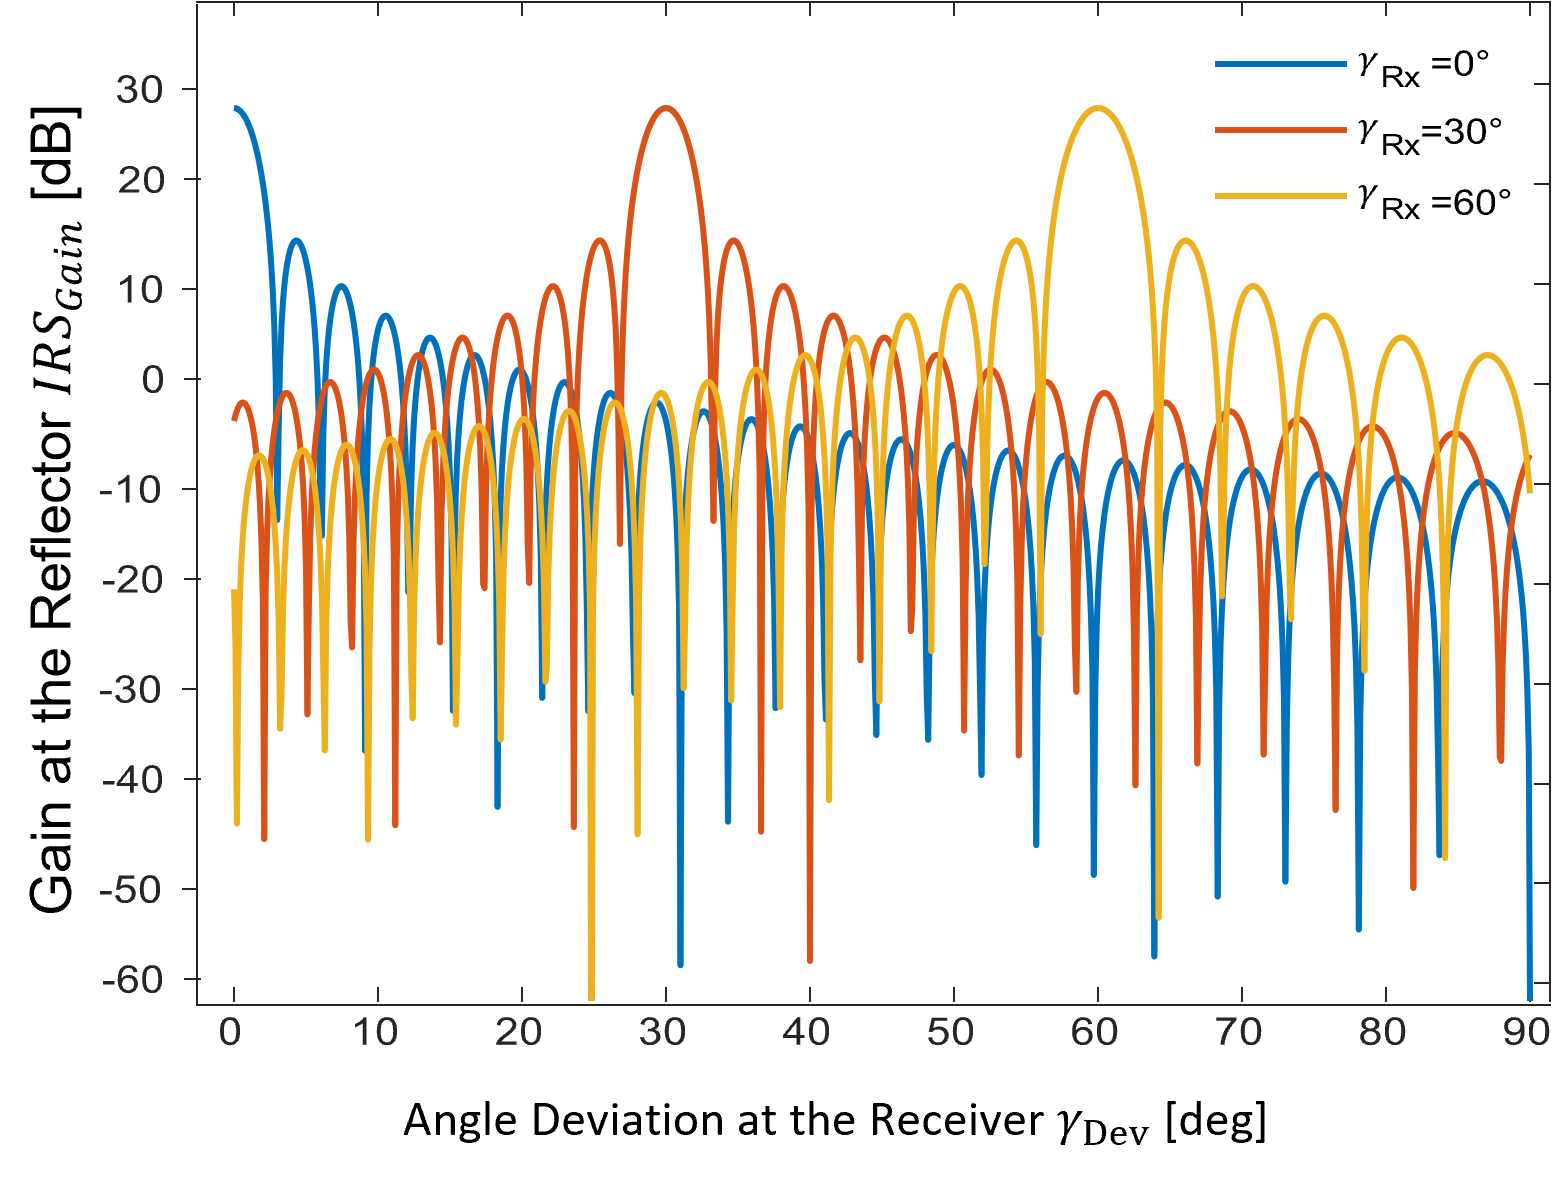
\includegraphics[width=0.7\linewidth]{images/Section 2 Images/model1_pattern}
	\caption{Gain at the reflector depicting the support of radiation pattern in \cite{8936989} when sweeping along the receiver i.e., $\gamma_{Rx} \neq \gamma_{Dev}$ for different placement of the receiver $\gamma_{Rx}$. A notable peak is observed for each $\gamma_{Rx}$ curve and the curve gradually decreases after this point. Additional parameters, $a=b=50\cdot \lambda$ at \SI{28}{\giga\hertz} frequency and $\theta_{Tx}=\varphi_{Tx}=0^\circ$. }
	\label{fig:model1pattern}
\end{figure}

All of these derivations of \ac{IRS} models are based on the Radar Cross Section which we discuss later in \Cref{Analytical Modeling of HELIOS Modules}. 
\section{Scope of Thesis} \label{Related Work or Scope of Thesis}
The previous sections have provided a thorough background on mmWave communications and particularly motivated the need for reflecting surfaces. Metasurfaces in the form of IRSs have risen as a hot topic in 6G research \cite{Scope_1, Scope_2, Scope_3, Scope_4}. Consequently, according end-to-end channel models have been developed.

As we have pointed out in this section, passive reflectors such as in the form of HELIOS reflectors are an alternative solution that comes with advantages in terms of compatibility with existing communication standards and zero-energy consumption. An analytical description for such is of utmost importance to realize HELIOS-enabled mmWave communications. Likewise, the goal of this master thesis is to derive such a description and compare it with the above IRS models. Similar to existing works, we aim to showcase the benefits of this model, particularly by using it in the context of an urban sample mmWave deployment scenario.